\section{Comparing device manufacturers, device models and network operators}
\label{sec:security_scoring}\label{sec:exp:security_score}

To allow buyers of Android devices to purchase those devices which have the best security they need to know how different device manufacturers, device models and network operators compare in terms of the security they provide.
We propose a method to score a device manufacturer, device model or network operator based on its historic performance at keeping devices up-to-date and fixing security vulnerabilities.
We find that Android as a whole gets a score of \daSecurityScore\ out of 10, the highest scoring device manufacturer is \emph{\daSecScoreBestmanufacturer} (\daSecScoreBestmanufacturerScore\ out of 10) and the lowest scoring is \emph{\daSecScoreWorstmanufacturer} (\daSecScoreWorstmanufacturerScore\ out of 10).

\subsection{Method: Scoring for security}\label{sec:security_scoring:method}

Computing how good a particular device manufacturer or device model is from a security standpoint is difficult as it depends on a number of factors which are hard to observe, particularly on a large scale.
Ideally we would consider both the prevalence of potential problems which were not exploited and actual security failures.
%\footnote{A perfectly secure operating system would among other things detect and prevent all phishing attacks, provide perfect principle of least privilege isolation, not have any vulnerabilities, instantly fix all discovered vulnerabilities, not allow any user data to be used in a way which the user does not approve of and be really easy for an ordinary person to use.}
However in the absence of such data we propose a scheme for assigning a device a score out of ten based on data which can be observed, is based on previous metrics, and which we expect correlates with the actual security of the devices.

The FUM score is computed from three components:
\begin{description}
  \item[free $f$] The proportion of running devices which were free from critical vulnerabilities over time. This is equivalent to Acer and Jackson's proposal to measure the security based on the proportion of users with at least one unpatched critical vulnerability~\cite{Acer2010} and similar to the Vulnerability Free Days (VFD) score~\cite{Wright2014}.
  Unlike VFD this is the proportion of running devices which were free from critical vulnerabilities over time, rather than days which the device manufacturer was free from outstanding critical vulnerabilities as that does not take account of the update process.
  \item[update $u$] The proportion of devices which run the latest version of Android shipped to any device produced by that device manufacturer. This is a measure of internal updatedness, a low score would mean many devices are being left behind.
  This assumes that newer versions are better with stronger security.
  Historically steps have been taken to improve Android security in newer versions so this assumption should generally hold, but sometimes new updates introduce new vulnerabilities.
  \item[mean $m$] The mean number of outstanding vulnerabilities affecting devices not fixed on any device shipped by the device manufacturer. This is related to the Median Active Vulnerabilities (MAV) measure~\cite{Wright2014} but is the mean rather than the median, as this gives a continuous value.
  An example is given in Figure~\ref{fig:mcalculation}.
%TODO should we compute the median instead?
\end{description}

\begin{figure}
\centering
%\includegraphics[width=\columnwidth]{figures/mcalculation}
% Graphic for TeX using PGF
% Title: /home/drt24/git/papers/da/securityupdates/figures/mcalculation.dia
% Creator: Dia v0.97.3
% CreationDate: Wed Apr 22 15:03:07 2015
% For: drt24
% \usepackage{tikz}
% The following commands are not supported in PSTricks at present
% We define them conditionally, so when they are implemented,
% this pgf file will use them.
\ifx\du\undefined
  \newlength{\du}
\fi
\setlength{\du}{5\unitlength}
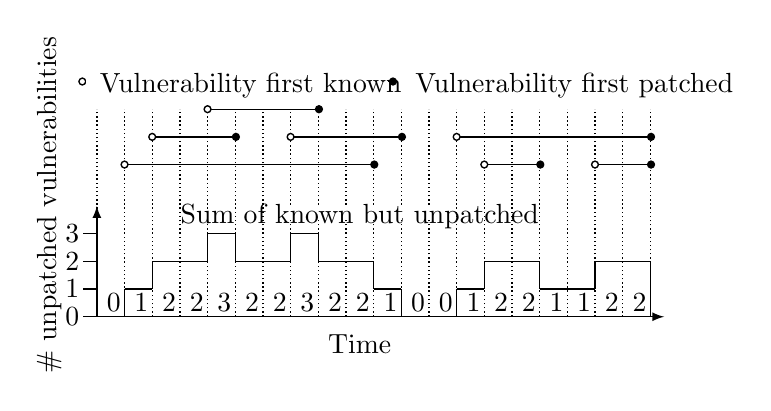
\begin{tikzpicture}
\pgftransformxscale{1.000000}
\pgftransformyscale{-1.000000}
\definecolor{dialinecolor}{rgb}{0.000000, 0.000000, 0.000000}
\pgfsetstrokecolor{dialinecolor}
\definecolor{dialinecolor}{rgb}{1.000000, 1.000000, 1.000000}
\pgfsetfillcolor{dialinecolor}
\pgfsetlinewidth{0.100000\du}
\pgfsetdash{{\pgflinewidth}{0.200000\du}}{0cm}
\pgfsetdash{{\pgflinewidth}{0.200000\du}}{0cm}
\pgfsetbuttcap
{
\definecolor{dialinecolor}{rgb}{0.000000, 0.000000, 0.000000}
\pgfsetfillcolor{dialinecolor}
% was here!!!
\definecolor{dialinecolor}{rgb}{0.000000, 0.000000, 0.000000}
\pgfsetstrokecolor{dialinecolor}
\draw (5.000000\du,24.000000\du)--(5.000000\du,9.000000\du);
}
\pgfsetlinewidth{0.100000\du}
\pgfsetdash{{\pgflinewidth}{0.200000\du}}{0cm}
\pgfsetdash{{\pgflinewidth}{0.200000\du}}{0cm}
\pgfsetbuttcap
{
\definecolor{dialinecolor}{rgb}{0.000000, 0.000000, 0.000000}
\pgfsetfillcolor{dialinecolor}
% was here!!!
\definecolor{dialinecolor}{rgb}{0.000000, 0.000000, 0.000000}
\pgfsetstrokecolor{dialinecolor}
\draw (7.000000\du,24.000000\du)--(7.000000\du,9.000000\du);
}
\pgfsetlinewidth{0.100000\du}
\pgfsetdash{{\pgflinewidth}{0.200000\du}}{0cm}
\pgfsetdash{{\pgflinewidth}{0.200000\du}}{0cm}
\pgfsetbuttcap
{
\definecolor{dialinecolor}{rgb}{0.000000, 0.000000, 0.000000}
\pgfsetfillcolor{dialinecolor}
% was here!!!
\definecolor{dialinecolor}{rgb}{0.000000, 0.000000, 0.000000}
\pgfsetstrokecolor{dialinecolor}
\draw (9.000000\du,24.000000\du)--(9.000000\du,9.000000\du);
}
\pgfsetlinewidth{0.100000\du}
\pgfsetdash{{\pgflinewidth}{0.200000\du}}{0cm}
\pgfsetdash{{\pgflinewidth}{0.200000\du}}{0cm}
\pgfsetbuttcap
{
\definecolor{dialinecolor}{rgb}{0.000000, 0.000000, 0.000000}
\pgfsetfillcolor{dialinecolor}
% was here!!!
\definecolor{dialinecolor}{rgb}{0.000000, 0.000000, 0.000000}
\pgfsetstrokecolor{dialinecolor}
\draw (11.000000\du,24.000000\du)--(11.000000\du,9.000000\du);
}
\pgfsetlinewidth{0.100000\du}
\pgfsetdash{{\pgflinewidth}{0.200000\du}}{0cm}
\pgfsetdash{{\pgflinewidth}{0.200000\du}}{0cm}
\pgfsetbuttcap
{
\definecolor{dialinecolor}{rgb}{0.000000, 0.000000, 0.000000}
\pgfsetfillcolor{dialinecolor}
% was here!!!
\definecolor{dialinecolor}{rgb}{0.000000, 0.000000, 0.000000}
\pgfsetstrokecolor{dialinecolor}
\draw (13.000000\du,24.000000\du)--(13.000000\du,9.000000\du);
}
\pgfsetlinewidth{0.100000\du}
\pgfsetdash{{\pgflinewidth}{0.200000\du}}{0cm}
\pgfsetdash{{\pgflinewidth}{0.200000\du}}{0cm}
\pgfsetbuttcap
{
\definecolor{dialinecolor}{rgb}{0.000000, 0.000000, 0.000000}
\pgfsetfillcolor{dialinecolor}
% was here!!!
\definecolor{dialinecolor}{rgb}{0.000000, 0.000000, 0.000000}
\pgfsetstrokecolor{dialinecolor}
\draw (15.000000\du,24.000000\du)--(15.000000\du,9.000000\du);
}
\pgfsetlinewidth{0.100000\du}
\pgfsetdash{{\pgflinewidth}{0.200000\du}}{0cm}
\pgfsetdash{{\pgflinewidth}{0.200000\du}}{0cm}
\pgfsetbuttcap
{
\definecolor{dialinecolor}{rgb}{0.000000, 0.000000, 0.000000}
\pgfsetfillcolor{dialinecolor}
% was here!!!
\definecolor{dialinecolor}{rgb}{0.000000, 0.000000, 0.000000}
\pgfsetstrokecolor{dialinecolor}
\draw (17.000000\du,24.000000\du)--(17.000000\du,9.000000\du);
}
\pgfsetlinewidth{0.100000\du}
\pgfsetdash{{\pgflinewidth}{0.200000\du}}{0cm}
\pgfsetdash{{\pgflinewidth}{0.200000\du}}{0cm}
\pgfsetbuttcap
{
\definecolor{dialinecolor}{rgb}{0.000000, 0.000000, 0.000000}
\pgfsetfillcolor{dialinecolor}
% was here!!!
\definecolor{dialinecolor}{rgb}{0.000000, 0.000000, 0.000000}
\pgfsetstrokecolor{dialinecolor}
\draw (19.000000\du,24.000000\du)--(19.000000\du,9.000000\du);
}
\pgfsetlinewidth{0.100000\du}
\pgfsetdash{{\pgflinewidth}{0.200000\du}}{0cm}
\pgfsetdash{{\pgflinewidth}{0.200000\du}}{0cm}
\pgfsetbuttcap
{
\definecolor{dialinecolor}{rgb}{0.000000, 0.000000, 0.000000}
\pgfsetfillcolor{dialinecolor}
% was here!!!
\definecolor{dialinecolor}{rgb}{0.000000, 0.000000, 0.000000}
\pgfsetstrokecolor{dialinecolor}
\draw (21.000000\du,24.000000\du)--(21.000000\du,9.000000\du);
}
\pgfsetlinewidth{0.100000\du}
\pgfsetdash{{\pgflinewidth}{0.200000\du}}{0cm}
\pgfsetdash{{\pgflinewidth}{0.200000\du}}{0cm}
\pgfsetbuttcap
{
\definecolor{dialinecolor}{rgb}{0.000000, 0.000000, 0.000000}
\pgfsetfillcolor{dialinecolor}
% was here!!!
\definecolor{dialinecolor}{rgb}{0.000000, 0.000000, 0.000000}
\pgfsetstrokecolor{dialinecolor}
\draw (23.000000\du,24.000000\du)--(23.000000\du,9.000000\du);
}
\pgfsetlinewidth{0.100000\du}
\pgfsetdash{{\pgflinewidth}{0.200000\du}}{0cm}
\pgfsetdash{{\pgflinewidth}{0.200000\du}}{0cm}
\pgfsetbuttcap
{
\definecolor{dialinecolor}{rgb}{0.000000, 0.000000, 0.000000}
\pgfsetfillcolor{dialinecolor}
% was here!!!
\definecolor{dialinecolor}{rgb}{0.000000, 0.000000, 0.000000}
\pgfsetstrokecolor{dialinecolor}
\draw (25.000000\du,24.000000\du)--(25.000000\du,9.000000\du);
}
\pgfsetlinewidth{0.100000\du}
\pgfsetdash{{\pgflinewidth}{0.200000\du}}{0cm}
\pgfsetdash{{\pgflinewidth}{0.200000\du}}{0cm}
\pgfsetbuttcap
{
\definecolor{dialinecolor}{rgb}{0.000000, 0.000000, 0.000000}
\pgfsetfillcolor{dialinecolor}
% was here!!!
\definecolor{dialinecolor}{rgb}{0.000000, 0.000000, 0.000000}
\pgfsetstrokecolor{dialinecolor}
\draw (27.000000\du,24.000000\du)--(27.000000\du,9.000000\du);
}
\pgfsetlinewidth{0.100000\du}
\pgfsetdash{{\pgflinewidth}{0.200000\du}}{0cm}
\pgfsetdash{{\pgflinewidth}{0.200000\du}}{0cm}
\pgfsetbuttcap
{
\definecolor{dialinecolor}{rgb}{0.000000, 0.000000, 0.000000}
\pgfsetfillcolor{dialinecolor}
% was here!!!
\definecolor{dialinecolor}{rgb}{0.000000, 0.000000, 0.000000}
\pgfsetstrokecolor{dialinecolor}
\draw (29.000000\du,24.000000\du)--(29.000000\du,9.000000\du);
}
\pgfsetlinewidth{0.100000\du}
\pgfsetdash{{\pgflinewidth}{0.200000\du}}{0cm}
\pgfsetdash{{\pgflinewidth}{0.200000\du}}{0cm}
\pgfsetbuttcap
{
\definecolor{dialinecolor}{rgb}{0.000000, 0.000000, 0.000000}
\pgfsetfillcolor{dialinecolor}
% was here!!!
\definecolor{dialinecolor}{rgb}{0.000000, 0.000000, 0.000000}
\pgfsetstrokecolor{dialinecolor}
\draw (31.000000\du,24.000000\du)--(31.000000\du,9.000000\du);
}
\pgfsetlinewidth{0.100000\du}
\pgfsetdash{}{0pt}
\pgfsetdash{}{0pt}
\pgfsetbuttcap
{
\definecolor{dialinecolor}{rgb}{0.000000, 0.000000, 0.000000}
\pgfsetfillcolor{dialinecolor}
% was here!!!
\pgfsetarrowsend{latex}
\definecolor{dialinecolor}{rgb}{0.000000, 0.000000, 0.000000}
\pgfsetstrokecolor{dialinecolor}
\draw (5.000000\du,24.000000\du)--(46.000000\du,24.000000\du);
}
\pgfsetlinewidth{0.100000\du}
\pgfsetdash{}{0pt}
\pgfsetdash{}{0pt}
\pgfsetbuttcap
{
\definecolor{dialinecolor}{rgb}{0.000000, 0.000000, 0.000000}
\pgfsetfillcolor{dialinecolor}
% was here!!!
}
\definecolor{dialinecolor}{rgb}{0.000000, 0.000000, 0.000000}
\pgfsetstrokecolor{dialinecolor}
\draw (7.250000\du,13.000000\du)--(25.300000\du,13.000000\du);
\pgfsetlinewidth{0.100000\du}
\pgfsetdash{}{0pt}
\pgfsetmiterjoin
\pgfsetbuttcap
\definecolor{dialinecolor}{rgb}{1.000000, 1.000000, 1.000000}
\pgfsetfillcolor{dialinecolor}
\pgfpathmoveto{\pgfpoint{6.750000\du}{13.000000\du}}
\pgfpathcurveto{\pgfpoint{6.750000\du}{12.875000\du}}{\pgfpoint{6.875000\du}{12.750000\du}}{\pgfpoint{7.000000\du}{12.750000\du}}
\pgfpathcurveto{\pgfpoint{7.125000\du}{12.750000\du}}{\pgfpoint{7.250000\du}{12.875000\du}}{\pgfpoint{7.250000\du}{13.000000\du}}
\pgfpathcurveto{\pgfpoint{7.250000\du}{13.125000\du}}{\pgfpoint{7.125000\du}{13.250000\du}}{\pgfpoint{7.000000\du}{13.250000\du}}
\pgfpathcurveto{\pgfpoint{6.875000\du}{13.250000\du}}{\pgfpoint{6.750000\du}{13.125000\du}}{\pgfpoint{6.750000\du}{13.000000\du}}
\pgfusepath{fill}
\definecolor{dialinecolor}{rgb}{0.000000, 0.000000, 0.000000}
\pgfsetstrokecolor{dialinecolor}
\pgfpathmoveto{\pgfpoint{6.750000\du}{13.000000\du}}
\pgfpathcurveto{\pgfpoint{6.750000\du}{12.875000\du}}{\pgfpoint{6.875000\du}{12.750000\du}}{\pgfpoint{7.000000\du}{12.750000\du}}
\pgfpathcurveto{\pgfpoint{7.125000\du}{12.750000\du}}{\pgfpoint{7.250000\du}{12.875000\du}}{\pgfpoint{7.250000\du}{13.000000\du}}
\pgfpathcurveto{\pgfpoint{7.250000\du}{13.125000\du}}{\pgfpoint{7.125000\du}{13.250000\du}}{\pgfpoint{7.000000\du}{13.250000\du}}
\pgfpathcurveto{\pgfpoint{6.875000\du}{13.250000\du}}{\pgfpoint{6.750000\du}{13.125000\du}}{\pgfpoint{6.750000\du}{13.000000\du}}
\pgfusepath{stroke}
\pgfsetlinewidth{0.100000\du}
\pgfsetdash{}{0pt}
\pgfsetmiterjoin
\pgfsetbuttcap
\definecolor{dialinecolor}{rgb}{0.000000, 0.000000, 0.000000}
\pgfsetfillcolor{dialinecolor}
\pgfpathmoveto{\pgfpoint{25.300000\du}{13.000000\du}}
\pgfpathcurveto{\pgfpoint{25.300000\du}{13.125000\du}}{\pgfpoint{25.175000\du}{13.250000\du}}{\pgfpoint{25.050000\du}{13.250000\du}}
\pgfpathcurveto{\pgfpoint{24.925000\du}{13.250000\du}}{\pgfpoint{24.800000\du}{13.125000\du}}{\pgfpoint{24.800000\du}{13.000000\du}}
\pgfpathcurveto{\pgfpoint{24.800000\du}{12.875000\du}}{\pgfpoint{24.925000\du}{12.750000\du}}{\pgfpoint{25.050000\du}{12.750000\du}}
\pgfpathcurveto{\pgfpoint{25.175000\du}{12.750000\du}}{\pgfpoint{25.300000\du}{12.875000\du}}{\pgfpoint{25.300000\du}{13.000000\du}}
\pgfusepath{fill}
\definecolor{dialinecolor}{rgb}{0.000000, 0.000000, 0.000000}
\pgfsetstrokecolor{dialinecolor}
\pgfpathmoveto{\pgfpoint{25.300000\du}{13.000000\du}}
\pgfpathcurveto{\pgfpoint{25.300000\du}{13.125000\du}}{\pgfpoint{25.175000\du}{13.250000\du}}{\pgfpoint{25.050000\du}{13.250000\du}}
\pgfpathcurveto{\pgfpoint{24.925000\du}{13.250000\du}}{\pgfpoint{24.800000\du}{13.125000\du}}{\pgfpoint{24.800000\du}{13.000000\du}}
\pgfpathcurveto{\pgfpoint{24.800000\du}{12.875000\du}}{\pgfpoint{24.925000\du}{12.750000\du}}{\pgfpoint{25.050000\du}{12.750000\du}}
\pgfpathcurveto{\pgfpoint{25.175000\du}{12.750000\du}}{\pgfpoint{25.300000\du}{12.875000\du}}{\pgfpoint{25.300000\du}{13.000000\du}}
\pgfusepath{stroke}
\pgfsetlinewidth{0.100000\du}
\pgfsetdash{}{0pt}
\pgfsetdash{}{0pt}
\pgfsetbuttcap
{
\definecolor{dialinecolor}{rgb}{0.000000, 0.000000, 0.000000}
\pgfsetfillcolor{dialinecolor}
% was here!!!
}
\definecolor{dialinecolor}{rgb}{0.000000, 0.000000, 0.000000}
\pgfsetstrokecolor{dialinecolor}
\draw (9.250000\du,11.000000\du)--(15.300000\du,11.000000\du);
\pgfsetlinewidth{0.100000\du}
\pgfsetdash{}{0pt}
\pgfsetmiterjoin
\pgfsetbuttcap
\definecolor{dialinecolor}{rgb}{1.000000, 1.000000, 1.000000}
\pgfsetfillcolor{dialinecolor}
\pgfpathmoveto{\pgfpoint{8.750000\du}{11.000000\du}}
\pgfpathcurveto{\pgfpoint{8.750000\du}{10.875000\du}}{\pgfpoint{8.875000\du}{10.750000\du}}{\pgfpoint{9.000000\du}{10.750000\du}}
\pgfpathcurveto{\pgfpoint{9.125000\du}{10.750000\du}}{\pgfpoint{9.250000\du}{10.875000\du}}{\pgfpoint{9.250000\du}{11.000000\du}}
\pgfpathcurveto{\pgfpoint{9.250000\du}{11.125000\du}}{\pgfpoint{9.125000\du}{11.250000\du}}{\pgfpoint{9.000000\du}{11.250000\du}}
\pgfpathcurveto{\pgfpoint{8.875000\du}{11.250000\du}}{\pgfpoint{8.750000\du}{11.125000\du}}{\pgfpoint{8.750000\du}{11.000000\du}}
\pgfusepath{fill}
\definecolor{dialinecolor}{rgb}{0.000000, 0.000000, 0.000000}
\pgfsetstrokecolor{dialinecolor}
\pgfpathmoveto{\pgfpoint{8.750000\du}{11.000000\du}}
\pgfpathcurveto{\pgfpoint{8.750000\du}{10.875000\du}}{\pgfpoint{8.875000\du}{10.750000\du}}{\pgfpoint{9.000000\du}{10.750000\du}}
\pgfpathcurveto{\pgfpoint{9.125000\du}{10.750000\du}}{\pgfpoint{9.250000\du}{10.875000\du}}{\pgfpoint{9.250000\du}{11.000000\du}}
\pgfpathcurveto{\pgfpoint{9.250000\du}{11.125000\du}}{\pgfpoint{9.125000\du}{11.250000\du}}{\pgfpoint{9.000000\du}{11.250000\du}}
\pgfpathcurveto{\pgfpoint{8.875000\du}{11.250000\du}}{\pgfpoint{8.750000\du}{11.125000\du}}{\pgfpoint{8.750000\du}{11.000000\du}}
\pgfusepath{stroke}
\pgfsetlinewidth{0.100000\du}
\pgfsetdash{}{0pt}
\pgfsetmiterjoin
\pgfsetbuttcap
\definecolor{dialinecolor}{rgb}{0.000000, 0.000000, 0.000000}
\pgfsetfillcolor{dialinecolor}
\pgfpathmoveto{\pgfpoint{15.300000\du}{11.000000\du}}
\pgfpathcurveto{\pgfpoint{15.300000\du}{11.125000\du}}{\pgfpoint{15.175000\du}{11.250000\du}}{\pgfpoint{15.050000\du}{11.250000\du}}
\pgfpathcurveto{\pgfpoint{14.925000\du}{11.250000\du}}{\pgfpoint{14.800000\du}{11.125000\du}}{\pgfpoint{14.800000\du}{11.000000\du}}
\pgfpathcurveto{\pgfpoint{14.800000\du}{10.875000\du}}{\pgfpoint{14.925000\du}{10.750000\du}}{\pgfpoint{15.050000\du}{10.750000\du}}
\pgfpathcurveto{\pgfpoint{15.175000\du}{10.750000\du}}{\pgfpoint{15.300000\du}{10.875000\du}}{\pgfpoint{15.300000\du}{11.000000\du}}
\pgfusepath{fill}
\definecolor{dialinecolor}{rgb}{0.000000, 0.000000, 0.000000}
\pgfsetstrokecolor{dialinecolor}
\pgfpathmoveto{\pgfpoint{15.300000\du}{11.000000\du}}
\pgfpathcurveto{\pgfpoint{15.300000\du}{11.125000\du}}{\pgfpoint{15.175000\du}{11.250000\du}}{\pgfpoint{15.050000\du}{11.250000\du}}
\pgfpathcurveto{\pgfpoint{14.925000\du}{11.250000\du}}{\pgfpoint{14.800000\du}{11.125000\du}}{\pgfpoint{14.800000\du}{11.000000\du}}
\pgfpathcurveto{\pgfpoint{14.800000\du}{10.875000\du}}{\pgfpoint{14.925000\du}{10.750000\du}}{\pgfpoint{15.050000\du}{10.750000\du}}
\pgfpathcurveto{\pgfpoint{15.175000\du}{10.750000\du}}{\pgfpoint{15.300000\du}{10.875000\du}}{\pgfpoint{15.300000\du}{11.000000\du}}
\pgfusepath{stroke}
\pgfsetlinewidth{0.100000\du}
\pgfsetdash{}{0pt}
\pgfsetdash{}{0pt}
\pgfsetbuttcap
{
\definecolor{dialinecolor}{rgb}{0.000000, 0.000000, 0.000000}
\pgfsetfillcolor{dialinecolor}
% was here!!!
}
\definecolor{dialinecolor}{rgb}{0.000000, 0.000000, 0.000000}
\pgfsetstrokecolor{dialinecolor}
\draw (13.250000\du,9.000000\du)--(21.300000\du,9.000000\du);
\pgfsetlinewidth{0.100000\du}
\pgfsetdash{}{0pt}
\pgfsetmiterjoin
\pgfsetbuttcap
\definecolor{dialinecolor}{rgb}{1.000000, 1.000000, 1.000000}
\pgfsetfillcolor{dialinecolor}
\pgfpathmoveto{\pgfpoint{12.750000\du}{9.000000\du}}
\pgfpathcurveto{\pgfpoint{12.750000\du}{8.875000\du}}{\pgfpoint{12.875000\du}{8.750000\du}}{\pgfpoint{13.000000\du}{8.750000\du}}
\pgfpathcurveto{\pgfpoint{13.125000\du}{8.750000\du}}{\pgfpoint{13.250000\du}{8.875000\du}}{\pgfpoint{13.250000\du}{9.000000\du}}
\pgfpathcurveto{\pgfpoint{13.250000\du}{9.125000\du}}{\pgfpoint{13.125000\du}{9.250000\du}}{\pgfpoint{13.000000\du}{9.250000\du}}
\pgfpathcurveto{\pgfpoint{12.875000\du}{9.250000\du}}{\pgfpoint{12.750000\du}{9.125000\du}}{\pgfpoint{12.750000\du}{9.000000\du}}
\pgfusepath{fill}
\definecolor{dialinecolor}{rgb}{0.000000, 0.000000, 0.000000}
\pgfsetstrokecolor{dialinecolor}
\pgfpathmoveto{\pgfpoint{12.750000\du}{9.000000\du}}
\pgfpathcurveto{\pgfpoint{12.750000\du}{8.875000\du}}{\pgfpoint{12.875000\du}{8.750000\du}}{\pgfpoint{13.000000\du}{8.750000\du}}
\pgfpathcurveto{\pgfpoint{13.125000\du}{8.750000\du}}{\pgfpoint{13.250000\du}{8.875000\du}}{\pgfpoint{13.250000\du}{9.000000\du}}
\pgfpathcurveto{\pgfpoint{13.250000\du}{9.125000\du}}{\pgfpoint{13.125000\du}{9.250000\du}}{\pgfpoint{13.000000\du}{9.250000\du}}
\pgfpathcurveto{\pgfpoint{12.875000\du}{9.250000\du}}{\pgfpoint{12.750000\du}{9.125000\du}}{\pgfpoint{12.750000\du}{9.000000\du}}
\pgfusepath{stroke}
\pgfsetlinewidth{0.100000\du}
\pgfsetdash{}{0pt}
\pgfsetmiterjoin
\pgfsetbuttcap
\definecolor{dialinecolor}{rgb}{0.000000, 0.000000, 0.000000}
\pgfsetfillcolor{dialinecolor}
\pgfpathmoveto{\pgfpoint{21.300000\du}{9.000000\du}}
\pgfpathcurveto{\pgfpoint{21.300000\du}{9.125000\du}}{\pgfpoint{21.175000\du}{9.250000\du}}{\pgfpoint{21.050000\du}{9.250000\du}}
\pgfpathcurveto{\pgfpoint{20.925000\du}{9.250000\du}}{\pgfpoint{20.800000\du}{9.125000\du}}{\pgfpoint{20.800000\du}{9.000000\du}}
\pgfpathcurveto{\pgfpoint{20.800000\du}{8.875000\du}}{\pgfpoint{20.925000\du}{8.750000\du}}{\pgfpoint{21.050000\du}{8.750000\du}}
\pgfpathcurveto{\pgfpoint{21.175000\du}{8.750000\du}}{\pgfpoint{21.300000\du}{8.875000\du}}{\pgfpoint{21.300000\du}{9.000000\du}}
\pgfusepath{fill}
\definecolor{dialinecolor}{rgb}{0.000000, 0.000000, 0.000000}
\pgfsetstrokecolor{dialinecolor}
\pgfpathmoveto{\pgfpoint{21.300000\du}{9.000000\du}}
\pgfpathcurveto{\pgfpoint{21.300000\du}{9.125000\du}}{\pgfpoint{21.175000\du}{9.250000\du}}{\pgfpoint{21.050000\du}{9.250000\du}}
\pgfpathcurveto{\pgfpoint{20.925000\du}{9.250000\du}}{\pgfpoint{20.800000\du}{9.125000\du}}{\pgfpoint{20.800000\du}{9.000000\du}}
\pgfpathcurveto{\pgfpoint{20.800000\du}{8.875000\du}}{\pgfpoint{20.925000\du}{8.750000\du}}{\pgfpoint{21.050000\du}{8.750000\du}}
\pgfpathcurveto{\pgfpoint{21.175000\du}{8.750000\du}}{\pgfpoint{21.300000\du}{8.875000\du}}{\pgfpoint{21.300000\du}{9.000000\du}}
\pgfusepath{stroke}
\pgfsetlinewidth{0.100000\du}
\pgfsetdash{}{0pt}
\pgfsetdash{}{0pt}
\pgfsetbuttcap
{
\definecolor{dialinecolor}{rgb}{0.000000, 0.000000, 0.000000}
\pgfsetfillcolor{dialinecolor}
% was here!!!
}
\definecolor{dialinecolor}{rgb}{0.000000, 0.000000, 0.000000}
\pgfsetstrokecolor{dialinecolor}
\draw (19.250000\du,11.000000\du)--(27.300000\du,11.000000\du);
\pgfsetlinewidth{0.100000\du}
\pgfsetdash{}{0pt}
\pgfsetmiterjoin
\pgfsetbuttcap
\definecolor{dialinecolor}{rgb}{1.000000, 1.000000, 1.000000}
\pgfsetfillcolor{dialinecolor}
\pgfpathmoveto{\pgfpoint{18.750000\du}{11.000000\du}}
\pgfpathcurveto{\pgfpoint{18.750000\du}{10.875000\du}}{\pgfpoint{18.875000\du}{10.750000\du}}{\pgfpoint{19.000000\du}{10.750000\du}}
\pgfpathcurveto{\pgfpoint{19.125000\du}{10.750000\du}}{\pgfpoint{19.250000\du}{10.875000\du}}{\pgfpoint{19.250000\du}{11.000000\du}}
\pgfpathcurveto{\pgfpoint{19.250000\du}{11.125000\du}}{\pgfpoint{19.125000\du}{11.250000\du}}{\pgfpoint{19.000000\du}{11.250000\du}}
\pgfpathcurveto{\pgfpoint{18.875000\du}{11.250000\du}}{\pgfpoint{18.750000\du}{11.125000\du}}{\pgfpoint{18.750000\du}{11.000000\du}}
\pgfusepath{fill}
\definecolor{dialinecolor}{rgb}{0.000000, 0.000000, 0.000000}
\pgfsetstrokecolor{dialinecolor}
\pgfpathmoveto{\pgfpoint{18.750000\du}{11.000000\du}}
\pgfpathcurveto{\pgfpoint{18.750000\du}{10.875000\du}}{\pgfpoint{18.875000\du}{10.750000\du}}{\pgfpoint{19.000000\du}{10.750000\du}}
\pgfpathcurveto{\pgfpoint{19.125000\du}{10.750000\du}}{\pgfpoint{19.250000\du}{10.875000\du}}{\pgfpoint{19.250000\du}{11.000000\du}}
\pgfpathcurveto{\pgfpoint{19.250000\du}{11.125000\du}}{\pgfpoint{19.125000\du}{11.250000\du}}{\pgfpoint{19.000000\du}{11.250000\du}}
\pgfpathcurveto{\pgfpoint{18.875000\du}{11.250000\du}}{\pgfpoint{18.750000\du}{11.125000\du}}{\pgfpoint{18.750000\du}{11.000000\du}}
\pgfusepath{stroke}
\pgfsetlinewidth{0.100000\du}
\pgfsetdash{}{0pt}
\pgfsetmiterjoin
\pgfsetbuttcap
\definecolor{dialinecolor}{rgb}{0.000000, 0.000000, 0.000000}
\pgfsetfillcolor{dialinecolor}
\pgfpathmoveto{\pgfpoint{27.300000\du}{11.000000\du}}
\pgfpathcurveto{\pgfpoint{27.300000\du}{11.125000\du}}{\pgfpoint{27.175000\du}{11.250000\du}}{\pgfpoint{27.050000\du}{11.250000\du}}
\pgfpathcurveto{\pgfpoint{26.925000\du}{11.250000\du}}{\pgfpoint{26.800000\du}{11.125000\du}}{\pgfpoint{26.800000\du}{11.000000\du}}
\pgfpathcurveto{\pgfpoint{26.800000\du}{10.875000\du}}{\pgfpoint{26.925000\du}{10.750000\du}}{\pgfpoint{27.050000\du}{10.750000\du}}
\pgfpathcurveto{\pgfpoint{27.175000\du}{10.750000\du}}{\pgfpoint{27.300000\du}{10.875000\du}}{\pgfpoint{27.300000\du}{11.000000\du}}
\pgfusepath{fill}
\definecolor{dialinecolor}{rgb}{0.000000, 0.000000, 0.000000}
\pgfsetstrokecolor{dialinecolor}
\pgfpathmoveto{\pgfpoint{27.300000\du}{11.000000\du}}
\pgfpathcurveto{\pgfpoint{27.300000\du}{11.125000\du}}{\pgfpoint{27.175000\du}{11.250000\du}}{\pgfpoint{27.050000\du}{11.250000\du}}
\pgfpathcurveto{\pgfpoint{26.925000\du}{11.250000\du}}{\pgfpoint{26.800000\du}{11.125000\du}}{\pgfpoint{26.800000\du}{11.000000\du}}
\pgfpathcurveto{\pgfpoint{26.800000\du}{10.875000\du}}{\pgfpoint{26.925000\du}{10.750000\du}}{\pgfpoint{27.050000\du}{10.750000\du}}
\pgfpathcurveto{\pgfpoint{27.175000\du}{10.750000\du}}{\pgfpoint{27.300000\du}{10.875000\du}}{\pgfpoint{27.300000\du}{11.000000\du}}
\pgfusepath{stroke}
\pgfsetlinewidth{0.100000\du}
\pgfsetdash{{\pgflinewidth}{0.200000\du}}{0cm}
\pgfsetdash{{\pgflinewidth}{0.200000\du}}{0cm}
\pgfsetbuttcap
{
\definecolor{dialinecolor}{rgb}{0.000000, 0.000000, 0.000000}
\pgfsetfillcolor{dialinecolor}
% was here!!!
\definecolor{dialinecolor}{rgb}{0.000000, 0.000000, 0.000000}
\pgfsetstrokecolor{dialinecolor}
\draw (33.000000\du,24.000000\du)--(33.000000\du,9.000000\du);
}
\pgfsetlinewidth{0.100000\du}
\pgfsetdash{{\pgflinewidth}{0.200000\du}}{0cm}
\pgfsetdash{{\pgflinewidth}{0.200000\du}}{0cm}
\pgfsetbuttcap
{
\definecolor{dialinecolor}{rgb}{0.000000, 0.000000, 0.000000}
\pgfsetfillcolor{dialinecolor}
% was here!!!
\definecolor{dialinecolor}{rgb}{0.000000, 0.000000, 0.000000}
\pgfsetstrokecolor{dialinecolor}
\draw (35.000000\du,24.000000\du)--(35.000000\du,9.000000\du);
}
\pgfsetlinewidth{0.100000\du}
\pgfsetdash{{\pgflinewidth}{0.200000\du}}{0cm}
\pgfsetdash{{\pgflinewidth}{0.200000\du}}{0cm}
\pgfsetbuttcap
{
\definecolor{dialinecolor}{rgb}{0.000000, 0.000000, 0.000000}
\pgfsetfillcolor{dialinecolor}
% was here!!!
\definecolor{dialinecolor}{rgb}{0.000000, 0.000000, 0.000000}
\pgfsetstrokecolor{dialinecolor}
\draw (37.000000\du,24.000000\du)--(37.000000\du,9.000000\du);
}
\pgfsetlinewidth{0.100000\du}
\pgfsetdash{{\pgflinewidth}{0.200000\du}}{0cm}
\pgfsetdash{{\pgflinewidth}{0.200000\du}}{0cm}
\pgfsetbuttcap
{
\definecolor{dialinecolor}{rgb}{0.000000, 0.000000, 0.000000}
\pgfsetfillcolor{dialinecolor}
% was here!!!
\definecolor{dialinecolor}{rgb}{0.000000, 0.000000, 0.000000}
\pgfsetstrokecolor{dialinecolor}
\draw (39.000000\du,24.000000\du)--(39.000000\du,9.000000\du);
}
\pgfsetlinewidth{0.100000\du}
\pgfsetdash{{\pgflinewidth}{0.200000\du}}{0cm}
\pgfsetdash{{\pgflinewidth}{0.200000\du}}{0cm}
\pgfsetbuttcap
{
\definecolor{dialinecolor}{rgb}{0.000000, 0.000000, 0.000000}
\pgfsetfillcolor{dialinecolor}
% was here!!!
\definecolor{dialinecolor}{rgb}{0.000000, 0.000000, 0.000000}
\pgfsetstrokecolor{dialinecolor}
\draw (41.000000\du,24.000000\du)--(41.000000\du,9.000000\du);
}
\pgfsetlinewidth{0.100000\du}
\pgfsetdash{{\pgflinewidth}{0.200000\du}}{0cm}
\pgfsetdash{{\pgflinewidth}{0.200000\du}}{0cm}
\pgfsetbuttcap
{
\definecolor{dialinecolor}{rgb}{0.000000, 0.000000, 0.000000}
\pgfsetfillcolor{dialinecolor}
% was here!!!
\definecolor{dialinecolor}{rgb}{0.000000, 0.000000, 0.000000}
\pgfsetstrokecolor{dialinecolor}
\draw (43.000000\du,24.000000\du)--(43.000000\du,9.000000\du);
}
\pgfsetlinewidth{0.100000\du}
\pgfsetdash{{\pgflinewidth}{0.200000\du}}{0cm}
\pgfsetdash{{\pgflinewidth}{0.200000\du}}{0cm}
\pgfsetbuttcap
{
\definecolor{dialinecolor}{rgb}{0.000000, 0.000000, 0.000000}
\pgfsetfillcolor{dialinecolor}
% was here!!!
\definecolor{dialinecolor}{rgb}{0.000000, 0.000000, 0.000000}
\pgfsetstrokecolor{dialinecolor}
\draw (45.000000\du,24.000000\du)--(45.000000\du,9.000000\du);
}
\pgfsetlinewidth{0.100000\du}
\pgfsetdash{}{0pt}
\pgfsetdash{}{0pt}
\pgfsetbuttcap
{
\definecolor{dialinecolor}{rgb}{0.000000, 0.000000, 0.000000}
\pgfsetfillcolor{dialinecolor}
% was here!!!
}
\definecolor{dialinecolor}{rgb}{0.000000, 0.000000, 0.000000}
\pgfsetstrokecolor{dialinecolor}
\draw (31.250000\du,11.000000\du)--(45.300000\du,11.000000\du);
\pgfsetlinewidth{0.100000\du}
\pgfsetdash{}{0pt}
\pgfsetmiterjoin
\pgfsetbuttcap
\definecolor{dialinecolor}{rgb}{1.000000, 1.000000, 1.000000}
\pgfsetfillcolor{dialinecolor}
\pgfpathmoveto{\pgfpoint{30.750000\du}{11.000000\du}}
\pgfpathcurveto{\pgfpoint{30.750000\du}{10.875000\du}}{\pgfpoint{30.875000\du}{10.750000\du}}{\pgfpoint{31.000000\du}{10.750000\du}}
\pgfpathcurveto{\pgfpoint{31.125000\du}{10.750000\du}}{\pgfpoint{31.250000\du}{10.875000\du}}{\pgfpoint{31.250000\du}{11.000000\du}}
\pgfpathcurveto{\pgfpoint{31.250000\du}{11.125000\du}}{\pgfpoint{31.125000\du}{11.250000\du}}{\pgfpoint{31.000000\du}{11.250000\du}}
\pgfpathcurveto{\pgfpoint{30.875000\du}{11.250000\du}}{\pgfpoint{30.750000\du}{11.125000\du}}{\pgfpoint{30.750000\du}{11.000000\du}}
\pgfusepath{fill}
\definecolor{dialinecolor}{rgb}{0.000000, 0.000000, 0.000000}
\pgfsetstrokecolor{dialinecolor}
\pgfpathmoveto{\pgfpoint{30.750000\du}{11.000000\du}}
\pgfpathcurveto{\pgfpoint{30.750000\du}{10.875000\du}}{\pgfpoint{30.875000\du}{10.750000\du}}{\pgfpoint{31.000000\du}{10.750000\du}}
\pgfpathcurveto{\pgfpoint{31.125000\du}{10.750000\du}}{\pgfpoint{31.250000\du}{10.875000\du}}{\pgfpoint{31.250000\du}{11.000000\du}}
\pgfpathcurveto{\pgfpoint{31.250000\du}{11.125000\du}}{\pgfpoint{31.125000\du}{11.250000\du}}{\pgfpoint{31.000000\du}{11.250000\du}}
\pgfpathcurveto{\pgfpoint{30.875000\du}{11.250000\du}}{\pgfpoint{30.750000\du}{11.125000\du}}{\pgfpoint{30.750000\du}{11.000000\du}}
\pgfusepath{stroke}
\pgfsetlinewidth{0.100000\du}
\pgfsetdash{}{0pt}
\pgfsetmiterjoin
\pgfsetbuttcap
\definecolor{dialinecolor}{rgb}{0.000000, 0.000000, 0.000000}
\pgfsetfillcolor{dialinecolor}
\pgfpathmoveto{\pgfpoint{45.300000\du}{11.000000\du}}
\pgfpathcurveto{\pgfpoint{45.300000\du}{11.125000\du}}{\pgfpoint{45.175000\du}{11.250000\du}}{\pgfpoint{45.050000\du}{11.250000\du}}
\pgfpathcurveto{\pgfpoint{44.925000\du}{11.250000\du}}{\pgfpoint{44.800000\du}{11.125000\du}}{\pgfpoint{44.800000\du}{11.000000\du}}
\pgfpathcurveto{\pgfpoint{44.800000\du}{10.875000\du}}{\pgfpoint{44.925000\du}{10.750000\du}}{\pgfpoint{45.050000\du}{10.750000\du}}
\pgfpathcurveto{\pgfpoint{45.175000\du}{10.750000\du}}{\pgfpoint{45.300000\du}{10.875000\du}}{\pgfpoint{45.300000\du}{11.000000\du}}
\pgfusepath{fill}
\definecolor{dialinecolor}{rgb}{0.000000, 0.000000, 0.000000}
\pgfsetstrokecolor{dialinecolor}
\pgfpathmoveto{\pgfpoint{45.300000\du}{11.000000\du}}
\pgfpathcurveto{\pgfpoint{45.300000\du}{11.125000\du}}{\pgfpoint{45.175000\du}{11.250000\du}}{\pgfpoint{45.050000\du}{11.250000\du}}
\pgfpathcurveto{\pgfpoint{44.925000\du}{11.250000\du}}{\pgfpoint{44.800000\du}{11.125000\du}}{\pgfpoint{44.800000\du}{11.000000\du}}
\pgfpathcurveto{\pgfpoint{44.800000\du}{10.875000\du}}{\pgfpoint{44.925000\du}{10.750000\du}}{\pgfpoint{45.050000\du}{10.750000\du}}
\pgfpathcurveto{\pgfpoint{45.175000\du}{10.750000\du}}{\pgfpoint{45.300000\du}{10.875000\du}}{\pgfpoint{45.300000\du}{11.000000\du}}
\pgfusepath{stroke}
\pgfsetlinewidth{0.100000\du}
\pgfsetdash{}{0pt}
\pgfsetdash{}{0pt}
\pgfsetbuttcap
{
\definecolor{dialinecolor}{rgb}{0.000000, 0.000000, 0.000000}
\pgfsetfillcolor{dialinecolor}
% was here!!!
}
\definecolor{dialinecolor}{rgb}{0.000000, 0.000000, 0.000000}
\pgfsetstrokecolor{dialinecolor}
\draw (33.250000\du,13.000000\du)--(37.300000\du,13.000000\du);
\pgfsetlinewidth{0.100000\du}
\pgfsetdash{}{0pt}
\pgfsetmiterjoin
\pgfsetbuttcap
\definecolor{dialinecolor}{rgb}{1.000000, 1.000000, 1.000000}
\pgfsetfillcolor{dialinecolor}
\pgfpathmoveto{\pgfpoint{32.750000\du}{13.000000\du}}
\pgfpathcurveto{\pgfpoint{32.750000\du}{12.875000\du}}{\pgfpoint{32.875000\du}{12.750000\du}}{\pgfpoint{33.000000\du}{12.750000\du}}
\pgfpathcurveto{\pgfpoint{33.125000\du}{12.750000\du}}{\pgfpoint{33.250000\du}{12.875000\du}}{\pgfpoint{33.250000\du}{13.000000\du}}
\pgfpathcurveto{\pgfpoint{33.250000\du}{13.125000\du}}{\pgfpoint{33.125000\du}{13.250000\du}}{\pgfpoint{33.000000\du}{13.250000\du}}
\pgfpathcurveto{\pgfpoint{32.875000\du}{13.250000\du}}{\pgfpoint{32.750000\du}{13.125000\du}}{\pgfpoint{32.750000\du}{13.000000\du}}
\pgfusepath{fill}
\definecolor{dialinecolor}{rgb}{0.000000, 0.000000, 0.000000}
\pgfsetstrokecolor{dialinecolor}
\pgfpathmoveto{\pgfpoint{32.750000\du}{13.000000\du}}
\pgfpathcurveto{\pgfpoint{32.750000\du}{12.875000\du}}{\pgfpoint{32.875000\du}{12.750000\du}}{\pgfpoint{33.000000\du}{12.750000\du}}
\pgfpathcurveto{\pgfpoint{33.125000\du}{12.750000\du}}{\pgfpoint{33.250000\du}{12.875000\du}}{\pgfpoint{33.250000\du}{13.000000\du}}
\pgfpathcurveto{\pgfpoint{33.250000\du}{13.125000\du}}{\pgfpoint{33.125000\du}{13.250000\du}}{\pgfpoint{33.000000\du}{13.250000\du}}
\pgfpathcurveto{\pgfpoint{32.875000\du}{13.250000\du}}{\pgfpoint{32.750000\du}{13.125000\du}}{\pgfpoint{32.750000\du}{13.000000\du}}
\pgfusepath{stroke}
\pgfsetlinewidth{0.100000\du}
\pgfsetdash{}{0pt}
\pgfsetmiterjoin
\pgfsetbuttcap
\definecolor{dialinecolor}{rgb}{0.000000, 0.000000, 0.000000}
\pgfsetfillcolor{dialinecolor}
\pgfpathmoveto{\pgfpoint{37.300000\du}{13.000000\du}}
\pgfpathcurveto{\pgfpoint{37.300000\du}{13.125000\du}}{\pgfpoint{37.175000\du}{13.250000\du}}{\pgfpoint{37.050000\du}{13.250000\du}}
\pgfpathcurveto{\pgfpoint{36.925000\du}{13.250000\du}}{\pgfpoint{36.800000\du}{13.125000\du}}{\pgfpoint{36.800000\du}{13.000000\du}}
\pgfpathcurveto{\pgfpoint{36.800000\du}{12.875000\du}}{\pgfpoint{36.925000\du}{12.750000\du}}{\pgfpoint{37.050000\du}{12.750000\du}}
\pgfpathcurveto{\pgfpoint{37.175000\du}{12.750000\du}}{\pgfpoint{37.300000\du}{12.875000\du}}{\pgfpoint{37.300000\du}{13.000000\du}}
\pgfusepath{fill}
\definecolor{dialinecolor}{rgb}{0.000000, 0.000000, 0.000000}
\pgfsetstrokecolor{dialinecolor}
\pgfpathmoveto{\pgfpoint{37.300000\du}{13.000000\du}}
\pgfpathcurveto{\pgfpoint{37.300000\du}{13.125000\du}}{\pgfpoint{37.175000\du}{13.250000\du}}{\pgfpoint{37.050000\du}{13.250000\du}}
\pgfpathcurveto{\pgfpoint{36.925000\du}{13.250000\du}}{\pgfpoint{36.800000\du}{13.125000\du}}{\pgfpoint{36.800000\du}{13.000000\du}}
\pgfpathcurveto{\pgfpoint{36.800000\du}{12.875000\du}}{\pgfpoint{36.925000\du}{12.750000\du}}{\pgfpoint{37.050000\du}{12.750000\du}}
\pgfpathcurveto{\pgfpoint{37.175000\du}{12.750000\du}}{\pgfpoint{37.300000\du}{12.875000\du}}{\pgfpoint{37.300000\du}{13.000000\du}}
\pgfusepath{stroke}
\pgfsetlinewidth{0.100000\du}
\pgfsetdash{}{0pt}
\pgfsetdash{}{0pt}
\pgfsetbuttcap
{
\definecolor{dialinecolor}{rgb}{0.000000, 0.000000, 0.000000}
\pgfsetfillcolor{dialinecolor}
% was here!!!
}
\definecolor{dialinecolor}{rgb}{0.000000, 0.000000, 0.000000}
\pgfsetstrokecolor{dialinecolor}
\draw (41.250000\du,13.000000\du)--(45.300000\du,13.000000\du);
\pgfsetlinewidth{0.100000\du}
\pgfsetdash{}{0pt}
\pgfsetmiterjoin
\pgfsetbuttcap
\definecolor{dialinecolor}{rgb}{1.000000, 1.000000, 1.000000}
\pgfsetfillcolor{dialinecolor}
\pgfpathmoveto{\pgfpoint{40.750000\du}{13.000000\du}}
\pgfpathcurveto{\pgfpoint{40.750000\du}{12.875000\du}}{\pgfpoint{40.875000\du}{12.750000\du}}{\pgfpoint{41.000000\du}{12.750000\du}}
\pgfpathcurveto{\pgfpoint{41.125000\du}{12.750000\du}}{\pgfpoint{41.250000\du}{12.875000\du}}{\pgfpoint{41.250000\du}{13.000000\du}}
\pgfpathcurveto{\pgfpoint{41.250000\du}{13.125000\du}}{\pgfpoint{41.125000\du}{13.250000\du}}{\pgfpoint{41.000000\du}{13.250000\du}}
\pgfpathcurveto{\pgfpoint{40.875000\du}{13.250000\du}}{\pgfpoint{40.750000\du}{13.125000\du}}{\pgfpoint{40.750000\du}{13.000000\du}}
\pgfusepath{fill}
\definecolor{dialinecolor}{rgb}{0.000000, 0.000000, 0.000000}
\pgfsetstrokecolor{dialinecolor}
\pgfpathmoveto{\pgfpoint{40.750000\du}{13.000000\du}}
\pgfpathcurveto{\pgfpoint{40.750000\du}{12.875000\du}}{\pgfpoint{40.875000\du}{12.750000\du}}{\pgfpoint{41.000000\du}{12.750000\du}}
\pgfpathcurveto{\pgfpoint{41.125000\du}{12.750000\du}}{\pgfpoint{41.250000\du}{12.875000\du}}{\pgfpoint{41.250000\du}{13.000000\du}}
\pgfpathcurveto{\pgfpoint{41.250000\du}{13.125000\du}}{\pgfpoint{41.125000\du}{13.250000\du}}{\pgfpoint{41.000000\du}{13.250000\du}}
\pgfpathcurveto{\pgfpoint{40.875000\du}{13.250000\du}}{\pgfpoint{40.750000\du}{13.125000\du}}{\pgfpoint{40.750000\du}{13.000000\du}}
\pgfusepath{stroke}
\pgfsetlinewidth{0.100000\du}
\pgfsetdash{}{0pt}
\pgfsetmiterjoin
\pgfsetbuttcap
\definecolor{dialinecolor}{rgb}{0.000000, 0.000000, 0.000000}
\pgfsetfillcolor{dialinecolor}
\pgfpathmoveto{\pgfpoint{45.300000\du}{13.000000\du}}
\pgfpathcurveto{\pgfpoint{45.300000\du}{13.125000\du}}{\pgfpoint{45.175000\du}{13.250000\du}}{\pgfpoint{45.050000\du}{13.250000\du}}
\pgfpathcurveto{\pgfpoint{44.925000\du}{13.250000\du}}{\pgfpoint{44.800000\du}{13.125000\du}}{\pgfpoint{44.800000\du}{13.000000\du}}
\pgfpathcurveto{\pgfpoint{44.800000\du}{12.875000\du}}{\pgfpoint{44.925000\du}{12.750000\du}}{\pgfpoint{45.050000\du}{12.750000\du}}
\pgfpathcurveto{\pgfpoint{45.175000\du}{12.750000\du}}{\pgfpoint{45.300000\du}{12.875000\du}}{\pgfpoint{45.300000\du}{13.000000\du}}
\pgfusepath{fill}
\definecolor{dialinecolor}{rgb}{0.000000, 0.000000, 0.000000}
\pgfsetstrokecolor{dialinecolor}
\pgfpathmoveto{\pgfpoint{45.300000\du}{13.000000\du}}
\pgfpathcurveto{\pgfpoint{45.300000\du}{13.125000\du}}{\pgfpoint{45.175000\du}{13.250000\du}}{\pgfpoint{45.050000\du}{13.250000\du}}
\pgfpathcurveto{\pgfpoint{44.925000\du}{13.250000\du}}{\pgfpoint{44.800000\du}{13.125000\du}}{\pgfpoint{44.800000\du}{13.000000\du}}
\pgfpathcurveto{\pgfpoint{44.800000\du}{12.875000\du}}{\pgfpoint{44.925000\du}{12.750000\du}}{\pgfpoint{45.050000\du}{12.750000\du}}
\pgfpathcurveto{\pgfpoint{45.175000\du}{12.750000\du}}{\pgfpoint{45.300000\du}{12.875000\du}}{\pgfpoint{45.300000\du}{13.000000\du}}
\pgfusepath{stroke}
\pgfsetlinewidth{0.100000\du}
\pgfsetdash{}{0pt}
\pgfsetdash{}{0pt}
\pgfsetbuttcap
{
\definecolor{dialinecolor}{rgb}{0.000000, 0.000000, 0.000000}
\pgfsetfillcolor{dialinecolor}
% was here!!!
\definecolor{dialinecolor}{rgb}{0.000000, 0.000000, 0.000000}
\pgfsetstrokecolor{dialinecolor}
\draw (7.000000\du,24.000000\du)--(7.000000\du,22.000000\du);
}
\pgfsetlinewidth{0.100000\du}
\pgfsetdash{}{0pt}
\pgfsetdash{}{0pt}
\pgfsetbuttcap
{
\definecolor{dialinecolor}{rgb}{0.000000, 0.000000, 0.000000}
\pgfsetfillcolor{dialinecolor}
% was here!!!
\definecolor{dialinecolor}{rgb}{0.000000, 0.000000, 0.000000}
\pgfsetstrokecolor{dialinecolor}
\draw (9.000000\du,22.000000\du)--(9.000000\du,20.000000\du);
}
\pgfsetlinewidth{0.100000\du}
\pgfsetdash{}{0pt}
\pgfsetdash{}{0pt}
\pgfsetbuttcap
{
\definecolor{dialinecolor}{rgb}{0.000000, 0.000000, 0.000000}
\pgfsetfillcolor{dialinecolor}
% was here!!!
\definecolor{dialinecolor}{rgb}{0.000000, 0.000000, 0.000000}
\pgfsetstrokecolor{dialinecolor}
\draw (13.000000\du,20.000000\du)--(13.000000\du,18.000000\du);
}
\pgfsetlinewidth{0.100000\du}
\pgfsetdash{}{0pt}
\pgfsetdash{}{0pt}
\pgfsetbuttcap
{
\definecolor{dialinecolor}{rgb}{0.000000, 0.000000, 0.000000}
\pgfsetfillcolor{dialinecolor}
% was here!!!
\definecolor{dialinecolor}{rgb}{0.000000, 0.000000, 0.000000}
\pgfsetstrokecolor{dialinecolor}
\draw (7.000000\du,22.000000\du)--(9.000000\du,22.000000\du);
}
\pgfsetlinewidth{0.100000\du}
\pgfsetdash{}{0pt}
\pgfsetdash{}{0pt}
\pgfsetbuttcap
{
\definecolor{dialinecolor}{rgb}{0.000000, 0.000000, 0.000000}
\pgfsetfillcolor{dialinecolor}
% was here!!!
\definecolor{dialinecolor}{rgb}{0.000000, 0.000000, 0.000000}
\pgfsetstrokecolor{dialinecolor}
\draw (9.000000\du,20.000000\du)--(13.000000\du,20.000000\du);
}
\pgfsetlinewidth{0.100000\du}
\pgfsetdash{}{0pt}
\pgfsetdash{}{0pt}
\pgfsetbuttcap
{
\definecolor{dialinecolor}{rgb}{0.000000, 0.000000, 0.000000}
\pgfsetfillcolor{dialinecolor}
% was here!!!
\definecolor{dialinecolor}{rgb}{0.000000, 0.000000, 0.000000}
\pgfsetstrokecolor{dialinecolor}
\draw (13.000000\du,18.000000\du)--(15.000000\du,18.000000\du);
}
\pgfsetlinewidth{0.100000\du}
\pgfsetdash{}{0pt}
\pgfsetdash{}{0pt}
\pgfsetbuttcap
{
\definecolor{dialinecolor}{rgb}{0.000000, 0.000000, 0.000000}
\pgfsetfillcolor{dialinecolor}
% was here!!!
\definecolor{dialinecolor}{rgb}{0.000000, 0.000000, 0.000000}
\pgfsetstrokecolor{dialinecolor}
\draw (15.000000\du,20.000000\du)--(15.000000\du,18.000000\du);
}
\pgfsetlinewidth{0.100000\du}
\pgfsetdash{}{0pt}
\pgfsetdash{}{0pt}
\pgfsetbuttcap
{
\definecolor{dialinecolor}{rgb}{0.000000, 0.000000, 0.000000}
\pgfsetfillcolor{dialinecolor}
% was here!!!
\definecolor{dialinecolor}{rgb}{0.000000, 0.000000, 0.000000}
\pgfsetstrokecolor{dialinecolor}
\draw (15.000000\du,20.000000\du)--(19.000000\du,20.000000\du);
}
\pgfsetlinewidth{0.100000\du}
\pgfsetdash{}{0pt}
\pgfsetdash{}{0pt}
\pgfsetbuttcap
{
\definecolor{dialinecolor}{rgb}{0.000000, 0.000000, 0.000000}
\pgfsetfillcolor{dialinecolor}
% was here!!!
\definecolor{dialinecolor}{rgb}{0.000000, 0.000000, 0.000000}
\pgfsetstrokecolor{dialinecolor}
\draw (19.000000\du,20.000000\du)--(19.000000\du,18.000000\du);
}
\pgfsetlinewidth{0.100000\du}
\pgfsetdash{}{0pt}
\pgfsetdash{}{0pt}
\pgfsetbuttcap
{
\definecolor{dialinecolor}{rgb}{0.000000, 0.000000, 0.000000}
\pgfsetfillcolor{dialinecolor}
% was here!!!
\definecolor{dialinecolor}{rgb}{0.000000, 0.000000, 0.000000}
\pgfsetstrokecolor{dialinecolor}
\draw (19.000000\du,18.000000\du)--(21.000000\du,18.000000\du);
}
\pgfsetlinewidth{0.100000\du}
\pgfsetdash{}{0pt}
\pgfsetdash{}{0pt}
\pgfsetbuttcap
{
\definecolor{dialinecolor}{rgb}{0.000000, 0.000000, 0.000000}
\pgfsetfillcolor{dialinecolor}
% was here!!!
\definecolor{dialinecolor}{rgb}{0.000000, 0.000000, 0.000000}
\pgfsetstrokecolor{dialinecolor}
\draw (25.000000\du,22.000000\du)--(25.000000\du,20.000000\du);
}
\pgfsetlinewidth{0.100000\du}
\pgfsetdash{}{0pt}
\pgfsetdash{}{0pt}
\pgfsetbuttcap
{
\definecolor{dialinecolor}{rgb}{0.000000, 0.000000, 0.000000}
\pgfsetfillcolor{dialinecolor}
% was here!!!
\definecolor{dialinecolor}{rgb}{0.000000, 0.000000, 0.000000}
\pgfsetstrokecolor{dialinecolor}
\draw (21.000000\du,20.000000\du)--(21.000000\du,18.000000\du);
}
\pgfsetlinewidth{0.100000\du}
\pgfsetdash{}{0pt}
\pgfsetdash{}{0pt}
\pgfsetbuttcap
{
\definecolor{dialinecolor}{rgb}{0.000000, 0.000000, 0.000000}
\pgfsetfillcolor{dialinecolor}
% was here!!!
\definecolor{dialinecolor}{rgb}{0.000000, 0.000000, 0.000000}
\pgfsetstrokecolor{dialinecolor}
\draw (33.000000\du,20.000000\du)--(37.000000\du,20.000000\du);
}
\pgfsetlinewidth{0.100000\du}
\pgfsetdash{}{0pt}
\pgfsetdash{}{0pt}
\pgfsetbuttcap
{
\definecolor{dialinecolor}{rgb}{0.000000, 0.000000, 0.000000}
\pgfsetfillcolor{dialinecolor}
% was here!!!
\definecolor{dialinecolor}{rgb}{0.000000, 0.000000, 0.000000}
\pgfsetstrokecolor{dialinecolor}
\draw (21.000000\du,20.000000\du)--(25.000000\du,20.000000\du);
}
\pgfsetlinewidth{0.100000\du}
\pgfsetdash{}{0pt}
\pgfsetdash{}{0pt}
\pgfsetbuttcap
{
\definecolor{dialinecolor}{rgb}{0.000000, 0.000000, 0.000000}
\pgfsetfillcolor{dialinecolor}
% was here!!!
\definecolor{dialinecolor}{rgb}{0.000000, 0.000000, 0.000000}
\pgfsetstrokecolor{dialinecolor}
\draw (31.000000\du,22.000000\du)--(33.000000\du,22.000000\du);
}
\pgfsetlinewidth{0.100000\du}
\pgfsetdash{}{0pt}
\pgfsetdash{}{0pt}
\pgfsetbuttcap
{
\definecolor{dialinecolor}{rgb}{0.000000, 0.000000, 0.000000}
\pgfsetfillcolor{dialinecolor}
% was here!!!
\definecolor{dialinecolor}{rgb}{0.000000, 0.000000, 0.000000}
\pgfsetstrokecolor{dialinecolor}
\draw (25.000000\du,22.000000\du)--(27.000000\du,22.000000\du);
}
\pgfsetlinewidth{0.100000\du}
\pgfsetdash{}{0pt}
\pgfsetdash{}{0pt}
\pgfsetbuttcap
{
\definecolor{dialinecolor}{rgb}{0.000000, 0.000000, 0.000000}
\pgfsetfillcolor{dialinecolor}
% was here!!!
\definecolor{dialinecolor}{rgb}{0.000000, 0.000000, 0.000000}
\pgfsetstrokecolor{dialinecolor}
\draw (31.000000\du,24.000000\du)--(31.000000\du,22.000000\du);
}
\pgfsetlinewidth{0.100000\du}
\pgfsetdash{}{0pt}
\pgfsetdash{}{0pt}
\pgfsetbuttcap
{
\definecolor{dialinecolor}{rgb}{0.000000, 0.000000, 0.000000}
\pgfsetfillcolor{dialinecolor}
% was here!!!
\definecolor{dialinecolor}{rgb}{0.000000, 0.000000, 0.000000}
\pgfsetstrokecolor{dialinecolor}
\draw (27.000000\du,24.000000\du)--(27.000000\du,22.000000\du);
}
\pgfsetlinewidth{0.100000\du}
\pgfsetdash{}{0pt}
\pgfsetdash{}{0pt}
\pgfsetbuttcap
{
\definecolor{dialinecolor}{rgb}{0.000000, 0.000000, 0.000000}
\pgfsetfillcolor{dialinecolor}
% was here!!!
\definecolor{dialinecolor}{rgb}{0.000000, 0.000000, 0.000000}
\pgfsetstrokecolor{dialinecolor}
\draw (37.000000\du,22.000000\du)--(37.000000\du,20.000000\du);
}
\pgfsetlinewidth{0.100000\du}
\pgfsetdash{}{0pt}
\pgfsetdash{}{0pt}
\pgfsetbuttcap
{
\definecolor{dialinecolor}{rgb}{0.000000, 0.000000, 0.000000}
\pgfsetfillcolor{dialinecolor}
% was here!!!
\definecolor{dialinecolor}{rgb}{0.000000, 0.000000, 0.000000}
\pgfsetstrokecolor{dialinecolor}
\draw (33.000000\du,22.000000\du)--(33.000000\du,20.000000\du);
}
\pgfsetlinewidth{0.100000\du}
\pgfsetdash{}{0pt}
\pgfsetdash{}{0pt}
\pgfsetbuttcap
{
\definecolor{dialinecolor}{rgb}{0.000000, 0.000000, 0.000000}
\pgfsetfillcolor{dialinecolor}
% was here!!!
\definecolor{dialinecolor}{rgb}{0.000000, 0.000000, 0.000000}
\pgfsetstrokecolor{dialinecolor}
\draw (41.000000\du,20.000000\du)--(45.000000\du,20.000000\du);
}
\pgfsetlinewidth{0.100000\du}
\pgfsetdash{}{0pt}
\pgfsetdash{}{0pt}
\pgfsetbuttcap
{
\definecolor{dialinecolor}{rgb}{0.000000, 0.000000, 0.000000}
\pgfsetfillcolor{dialinecolor}
% was here!!!
\definecolor{dialinecolor}{rgb}{0.000000, 0.000000, 0.000000}
\pgfsetstrokecolor{dialinecolor}
\draw (37.000000\du,22.000000\du)--(41.000000\du,22.000000\du);
}
\pgfsetlinewidth{0.100000\du}
\pgfsetdash{}{0pt}
\pgfsetdash{}{0pt}
\pgfsetbuttcap
{
\definecolor{dialinecolor}{rgb}{0.000000, 0.000000, 0.000000}
\pgfsetfillcolor{dialinecolor}
% was here!!!
\definecolor{dialinecolor}{rgb}{0.000000, 0.000000, 0.000000}
\pgfsetstrokecolor{dialinecolor}
\draw (45.000000\du,24.000000\du)--(45.000000\du,20.000000\du);
}
\pgfsetlinewidth{0.100000\du}
\pgfsetdash{}{0pt}
\pgfsetdash{}{0pt}
\pgfsetbuttcap
{
\definecolor{dialinecolor}{rgb}{0.000000, 0.000000, 0.000000}
\pgfsetfillcolor{dialinecolor}
% was here!!!
\definecolor{dialinecolor}{rgb}{0.000000, 0.000000, 0.000000}
\pgfsetstrokecolor{dialinecolor}
\draw (41.000000\du,22.000000\du)--(41.000000\du,20.000000\du);
}
\pgfsetlinewidth{0.100000\du}
\pgfsetdash{}{0pt}
\pgfsetdash{}{0pt}
\pgfsetbuttcap
{
\definecolor{dialinecolor}{rgb}{0.000000, 0.000000, 0.000000}
\pgfsetfillcolor{dialinecolor}
% was here!!!
}
\definecolor{dialinecolor}{rgb}{0.000000, 0.000000, 0.000000}
\pgfsetstrokecolor{dialinecolor}
\draw (4.200000\du,7.000000\du)--(26.650000\du,7.000000\du);
\pgfsetlinewidth{0.100000\du}
\pgfsetdash{}{0pt}
\pgfsetmiterjoin
\pgfsetbuttcap
\definecolor{dialinecolor}{rgb}{1.000000, 1.000000, 1.000000}
\pgfsetfillcolor{dialinecolor}
\pgfpathmoveto{\pgfpoint{3.700000\du}{7.000000\du}}
\pgfpathcurveto{\pgfpoint{3.700000\du}{6.875000\du}}{\pgfpoint{3.825000\du}{6.750000\du}}{\pgfpoint{3.950000\du}{6.750000\du}}
\pgfpathcurveto{\pgfpoint{4.075000\du}{6.750000\du}}{\pgfpoint{4.200000\du}{6.875000\du}}{\pgfpoint{4.200000\du}{7.000000\du}}
\pgfpathcurveto{\pgfpoint{4.200000\du}{7.125000\du}}{\pgfpoint{4.075000\du}{7.250000\du}}{\pgfpoint{3.950000\du}{7.250000\du}}
\pgfpathcurveto{\pgfpoint{3.825000\du}{7.250000\du}}{\pgfpoint{3.700000\du}{7.125000\du}}{\pgfpoint{3.700000\du}{7.000000\du}}
\pgfusepath{fill}
\definecolor{dialinecolor}{rgb}{0.000000, 0.000000, 0.000000}
\pgfsetstrokecolor{dialinecolor}
\pgfpathmoveto{\pgfpoint{3.700000\du}{7.000000\du}}
\pgfpathcurveto{\pgfpoint{3.700000\du}{6.875000\du}}{\pgfpoint{3.825000\du}{6.750000\du}}{\pgfpoint{3.950000\du}{6.750000\du}}
\pgfpathcurveto{\pgfpoint{4.075000\du}{6.750000\du}}{\pgfpoint{4.200000\du}{6.875000\du}}{\pgfpoint{4.200000\du}{7.000000\du}}
\pgfpathcurveto{\pgfpoint{4.200000\du}{7.125000\du}}{\pgfpoint{4.075000\du}{7.250000\du}}{\pgfpoint{3.950000\du}{7.250000\du}}
\pgfpathcurveto{\pgfpoint{3.825000\du}{7.250000\du}}{\pgfpoint{3.700000\du}{7.125000\du}}{\pgfpoint{3.700000\du}{7.000000\du}}
\pgfusepath{stroke}
\pgfsetlinewidth{0.100000\du}
\pgfsetdash{}{0pt}
\pgfsetmiterjoin
\pgfsetbuttcap
\definecolor{dialinecolor}{rgb}{0.000000, 0.000000, 0.000000}
\pgfsetfillcolor{dialinecolor}
\pgfpathmoveto{\pgfpoint{26.650000\du}{7.000000\du}}
\pgfpathcurveto{\pgfpoint{26.650000\du}{7.125000\du}}{\pgfpoint{26.525000\du}{7.250000\du}}{\pgfpoint{26.400000\du}{7.250000\du}}
\pgfpathcurveto{\pgfpoint{26.275000\du}{7.250000\du}}{\pgfpoint{26.150000\du}{7.125000\du}}{\pgfpoint{26.150000\du}{7.000000\du}}
\pgfpathcurveto{\pgfpoint{26.150000\du}{6.875000\du}}{\pgfpoint{26.275000\du}{6.750000\du}}{\pgfpoint{26.400000\du}{6.750000\du}}
\pgfpathcurveto{\pgfpoint{26.525000\du}{6.750000\du}}{\pgfpoint{26.650000\du}{6.875000\du}}{\pgfpoint{26.650000\du}{7.000000\du}}
\pgfusepath{fill}
\definecolor{dialinecolor}{rgb}{0.000000, 0.000000, 0.000000}
\pgfsetstrokecolor{dialinecolor}
\pgfpathmoveto{\pgfpoint{26.650000\du}{7.000000\du}}
\pgfpathcurveto{\pgfpoint{26.650000\du}{7.125000\du}}{\pgfpoint{26.525000\du}{7.250000\du}}{\pgfpoint{26.400000\du}{7.250000\du}}
\pgfpathcurveto{\pgfpoint{26.275000\du}{7.250000\du}}{\pgfpoint{26.150000\du}{7.125000\du}}{\pgfpoint{26.150000\du}{7.000000\du}}
\pgfpathcurveto{\pgfpoint{26.150000\du}{6.875000\du}}{\pgfpoint{26.275000\du}{6.750000\du}}{\pgfpoint{26.400000\du}{6.750000\du}}
\pgfpathcurveto{\pgfpoint{26.525000\du}{6.750000\du}}{\pgfpoint{26.650000\du}{6.875000\du}}{\pgfpoint{26.650000\du}{7.000000\du}}
\pgfusepath{stroke}
\pgfsetlinewidth{0.400000\du}
\pgfsetdash{}{0pt}
\pgfsetdash{}{0pt}
\pgfsetbuttcap
{
\definecolor{dialinecolor}{rgb}{1.000000, 1.000000, 1.000000}
\pgfsetfillcolor{dialinecolor}
% was here!!!
\definecolor{dialinecolor}{rgb}{1.000000, 1.000000, 1.000000}
\pgfsetstrokecolor{dialinecolor}
\draw (4.250000\du,7.000000\du)--(26.050000\du,7.000000\du);
}
% setfont left to latex
\definecolor{dialinecolor}{rgb}{0.000000, 0.000000, 0.000000}
\pgfsetstrokecolor{dialinecolor}
\node[anchor=west] at (4.350000\du,7.293750\du){Vulnerability first known};
% setfont left to latex
\definecolor{dialinecolor}{rgb}{0.000000, 0.000000, 0.000000}
\pgfsetstrokecolor{dialinecolor}
\node[anchor=west] at (27.150000\du,7.293750\du){Vulnerability first patched};
% setfont left to latex
\definecolor{dialinecolor}{rgb}{0.000000, 0.000000, 0.000000}
\pgfsetstrokecolor{dialinecolor}
\node at (24.000000\du,26.000000\du){Time};
\definecolor{dialinecolor}{rgb}{1.000000, 1.000000, 1.000000}
\pgfsetfillcolor{dialinecolor}
\fill (17.748750\du,15.962500\du)--(17.748750\du,16.950000\du)--(30.251250\du,16.950000\du)--(30.251250\du,15.962500\du)--cycle;
% setfont left to latex
\definecolor{dialinecolor}{rgb}{0.000000, 0.000000, 0.000000}
\pgfsetstrokecolor{dialinecolor}
\node at (24.000000\du,16.750000\du){Sum of known but unpatched};
% setfont left to latex
\definecolor{dialinecolor}{rgb}{0.000000, 0.000000, 0.000000}
\pgfsetstrokecolor{dialinecolor}
\node[anchor=west] at (5.650000\du,22.800000\du){};
\pgfsetlinewidth{0.100000\du}
\pgfsetdash{}{0pt}
\pgfsetdash{}{0pt}
\pgfsetbuttcap
{
\definecolor{dialinecolor}{rgb}{0.000000, 0.000000, 0.000000}
\pgfsetfillcolor{dialinecolor}
% was here!!!
\pgfsetarrowsend{latex}
\definecolor{dialinecolor}{rgb}{0.000000, 0.000000, 0.000000}
\pgfsetstrokecolor{dialinecolor}
\draw (5.000000\du,24.000000\du)--(5.000000\du,16.000000\du);
}
\pgfsetlinewidth{0.100000\du}
\pgfsetdash{}{0pt}
\pgfsetdash{}{0pt}
\pgfsetbuttcap
{
\definecolor{dialinecolor}{rgb}{0.000000, 0.000000, 0.000000}
\pgfsetfillcolor{dialinecolor}
% was here!!!
\definecolor{dialinecolor}{rgb}{0.000000, 0.000000, 0.000000}
\pgfsetstrokecolor{dialinecolor}
\draw (5.000000\du,22.000000\du)--(4.000000\du,22.000000\du);
}
\pgfsetlinewidth{0.100000\du}
\pgfsetdash{}{0pt}
\pgfsetdash{}{0pt}
\pgfsetbuttcap
{
\definecolor{dialinecolor}{rgb}{0.000000, 0.000000, 0.000000}
\pgfsetfillcolor{dialinecolor}
% was here!!!
\definecolor{dialinecolor}{rgb}{0.000000, 0.000000, 0.000000}
\pgfsetstrokecolor{dialinecolor}
\draw (5.000000\du,20.000000\du)--(4.000000\du,20.000000\du);
}
\pgfsetlinewidth{0.100000\du}
\pgfsetdash{}{0pt}
\pgfsetdash{}{0pt}
\pgfsetbuttcap
{
\definecolor{dialinecolor}{rgb}{0.000000, 0.000000, 0.000000}
\pgfsetfillcolor{dialinecolor}
% was here!!!
\definecolor{dialinecolor}{rgb}{0.000000, 0.000000, 0.000000}
\pgfsetstrokecolor{dialinecolor}
\draw (5.000000\du,18.000000\du)--(4.000000\du,18.000000\du);
}
\pgfsetlinewidth{0.100000\du}
\pgfsetdash{}{0pt}
\pgfsetdash{}{0pt}
\pgfsetbuttcap
{
\definecolor{dialinecolor}{rgb}{0.000000, 0.000000, 0.000000}
\pgfsetfillcolor{dialinecolor}
% was here!!!
\definecolor{dialinecolor}{rgb}{0.000000, 0.000000, 0.000000}
\pgfsetstrokecolor{dialinecolor}
\draw (5.000000\du,24.000000\du)--(4.000000\du,24.000000\du);
}
% setfont left to latex
\definecolor{dialinecolor}{rgb}{0.000000, 0.000000, 0.000000}
\pgfsetstrokecolor{dialinecolor}
\node[anchor=west] at (2.000000\du,24.000000\du){0};
% setfont left to latex
\definecolor{dialinecolor}{rgb}{0.000000, 0.000000, 0.000000}
\pgfsetstrokecolor{dialinecolor}
\node[anchor=west] at (2.000000\du,22.000000\du){1};
% setfont left to latex
\definecolor{dialinecolor}{rgb}{0.000000, 0.000000, 0.000000}
\pgfsetstrokecolor{dialinecolor}
\node[anchor=west] at (2.000000\du,20.000000\du){2};
% setfont left to latex
\definecolor{dialinecolor}{rgb}{0.000000, 0.000000, 0.000000}
\pgfsetstrokecolor{dialinecolor}
\node[anchor=west] at (2.000000\du,18.000000\du){3};
% setfont left to latex
\definecolor{dialinecolor}{rgb}{0.000000, 0.000000, 0.000000}
\pgfsetstrokecolor{dialinecolor}
\node[anchor=west] at (-0.050000\du,15.950000\du){\rotatebox{90}{\# unpatched vulnerabilities}};
% setfont left to latex
\definecolor{dialinecolor}{rgb}{0.000000, 0.000000, 0.000000}
\pgfsetstrokecolor{dialinecolor}
\node[anchor=west] at (5.000000\du,27.000000\du){};
% setfont left to latex
\definecolor{dialinecolor}{rgb}{0.000000, 0.000000, 0.000000}
\pgfsetstrokecolor{dialinecolor}
\node[anchor=west] at (5.000000\du,23.000000\du){0};
% setfont left to latex
\definecolor{dialinecolor}{rgb}{0.000000, 0.000000, 0.000000}
\pgfsetstrokecolor{dialinecolor}
\node[anchor=west] at (27.000000\du,23.000000\du){0};
% setfont left to latex
\definecolor{dialinecolor}{rgb}{0.000000, 0.000000, 0.000000}
\pgfsetstrokecolor{dialinecolor}
\node[anchor=west] at (29.000000\du,23.000000\du){0};
% setfont left to latex
\definecolor{dialinecolor}{rgb}{0.000000, 0.000000, 0.000000}
\pgfsetstrokecolor{dialinecolor}
\node[anchor=west] at (7.000000\du,23.000000\du){1};
% setfont left to latex
\definecolor{dialinecolor}{rgb}{0.000000, 0.000000, 0.000000}
\pgfsetstrokecolor{dialinecolor}
\node[anchor=west] at (25.000000\du,23.000000\du){1};
% setfont left to latex
\definecolor{dialinecolor}{rgb}{0.000000, 0.000000, 0.000000}
\pgfsetstrokecolor{dialinecolor}
\node[anchor=west] at (31.000000\du,23.000000\du){1};
% setfont left to latex
\definecolor{dialinecolor}{rgb}{0.000000, 0.000000, 0.000000}
\pgfsetstrokecolor{dialinecolor}
\node[anchor=west] at (39.000000\du,23.000000\du){1};
% setfont left to latex
\definecolor{dialinecolor}{rgb}{0.000000, 0.000000, 0.000000}
\pgfsetstrokecolor{dialinecolor}
\node[anchor=west] at (37.000000\du,23.000000\du){1};
% setfont left to latex
\definecolor{dialinecolor}{rgb}{0.000000, 0.000000, 0.000000}
\pgfsetstrokecolor{dialinecolor}
\node[anchor=west] at (9.000000\du,23.000000\du){2};
% setfont left to latex
\definecolor{dialinecolor}{rgb}{0.000000, 0.000000, 0.000000}
\pgfsetstrokecolor{dialinecolor}
\node[anchor=west] at (11.000000\du,23.000000\du){2};
% setfont left to latex
\definecolor{dialinecolor}{rgb}{0.000000, 0.000000, 0.000000}
\pgfsetstrokecolor{dialinecolor}
\node[anchor=west] at (17.000000\du,23.000000\du){2};
% setfont left to latex
\definecolor{dialinecolor}{rgb}{0.000000, 0.000000, 0.000000}
\pgfsetstrokecolor{dialinecolor}
\node[anchor=west] at (15.000000\du,23.000000\du){2};
% setfont left to latex
\definecolor{dialinecolor}{rgb}{0.000000, 0.000000, 0.000000}
\pgfsetstrokecolor{dialinecolor}
\node[anchor=west] at (21.000000\du,23.000000\du){2};
% setfont left to latex
\definecolor{dialinecolor}{rgb}{0.000000, 0.000000, 0.000000}
\pgfsetstrokecolor{dialinecolor}
\node[anchor=west] at (23.000000\du,23.000000\du){2};
% setfont left to latex
\definecolor{dialinecolor}{rgb}{0.000000, 0.000000, 0.000000}
\pgfsetstrokecolor{dialinecolor}
\node[anchor=west] at (33.000000\du,23.000000\du){2};
% setfont left to latex
\definecolor{dialinecolor}{rgb}{0.000000, 0.000000, 0.000000}
\pgfsetstrokecolor{dialinecolor}
\node[anchor=west] at (35.000000\du,23.000000\du){2};
% setfont left to latex
\definecolor{dialinecolor}{rgb}{0.000000, 0.000000, 0.000000}
\pgfsetstrokecolor{dialinecolor}
\node[anchor=west] at (41.000000\du,23.000000\du){2};
% setfont left to latex
\definecolor{dialinecolor}{rgb}{0.000000, 0.000000, 0.000000}
\pgfsetstrokecolor{dialinecolor}
\node[anchor=west] at (43.000000\du,23.000000\du){2};
% setfont left to latex
\definecolor{dialinecolor}{rgb}{0.000000, 0.000000, 0.000000}
\pgfsetstrokecolor{dialinecolor}
\node[anchor=west] at (13.000000\du,23.000000\du){3};
% setfont left to latex
\definecolor{dialinecolor}{rgb}{0.000000, 0.000000, 0.000000}
\pgfsetstrokecolor{dialinecolor}
\node[anchor=west] at (19.000000\du,23.000000\du){3};
% setfont left to latex
\definecolor{dialinecolor}{rgb}{0.000000, 0.000000, 0.000000}
\pgfsetstrokecolor{dialinecolor}
\node[anchor=west] at (10.000000\du,21.000000\du){};
\end{tikzpicture}

\caption{As vulnerabilities are discovered and patched the sum of known but unpatched vulnerabilities each day varies. From this we can calculate $m = (0 \times 3 + 1 \times 5 + 2 \times 10 + 3 \times 2) / 20 = 1.55$ For comparison VFD = 0.15 and MAV = 2. Example based on the one given by Wright~\cite{Wright2014}.}
\label{fig:mcalculation}
\end{figure}

These three metrics $f$, $u$ and $m$ together measure the security of a platform with respect to known vulnerabilities and updates.
$f$ is a key measure of the direct risk to users as if there is any known but unfixed vulnerability then they are vulnerable.
However it does not capture the increased risk caused by there being multiple known vulnerabilities which gives an attacker more opportunities and increases the likelihood of a piece of malware having a matching exploit.
This is captured by the $m$ score which measures the size of the device manufacturers queue of outstanding vulnerabilities but does not take into account the update process or measure the actual end user security.
Neither of these metrics capture whether devices are being left behind and not being kept up-to-date with the most recent (and hopefully most secure) version which is captured by $u$.

We want to provide a score out of 10 as this is easy for phone buyers to understand as many ratings are given as a score out of 10.
Since $f$ is the most important metric we weight it more highly.
Since $m$ is an unbounded positive real number, we map it into the range [0--1).
This gives us Equation~\ref{eq:score}:

\begin{equation}
\mathrm{score} = 4 \cdot f + 3 \cdot u + 3 \cdot \frac{2}{1+e^m} \label{eq:score}
\end{equation}

We can compute the uncertainty for $f$, $u$ and $m$.
$f$ is computed by taking the total secure device days and dividing it by the total insecure and secure device days.
The total secure device days and total insecure device days are both counting experiments and so their measurement error is their square root~\cite{Taylor1997}.
Since the numbers involved are large, the uncertainty in $f$ is small.
$u$ is computed by taking the sum of the proportions of devices running the most recent version each day, both the count of devices running the maximum version and total count have square root uncertainties.
$m$ is computed by counting the number of vulnerabilities which affected that entity and which have not yet been fixed on any device we have observed from that entity every day and averaging over observed days.
However it could be that the entity has released a fix to some devices but we have not yet observed a device with that fix.
So the uncertainty in each vulnerability truly being outstanding is the probability of not having observed a fixed device if fixed device existed.
We assume that if the fix has been released then at least \daMeanOutstandingProbability\ of devices have the fix.
This gives an uncertainty of \daMeanOutstandingUncertaintyEquation\ where $n$ is the number of devices contributing to that day's data for each vulnerability outstanding each day.
The Python \texttt{uncertainties} library was used to propagate uncertainties through calculations.
This does not capture systematic errors such as those due to not including vulnerabilities which do affect devices, but for comparison that does not matter.
However we do not include manufacturer specific vulnerabilities which will influence comparisons, but we expect that performance in fixing manufacturer specific vulnerabilities is strongly correlated with performance fixing vulnerabilities affecting all of Android.

\todolater{There must be some way of putting an error bound on our results by considering the error on the whole DA set and the size of the subset used for each device manufacturer and device model}

\subsection{Results: Security scores}\label{sec:security_scoring:results}
The scores across the whole of Android are that \daMeanInsecurityPerc\ of devices are exposed to known root exploits.
There are on average \daMeanOutstandingVulnerabilities\ outstanding vulnerabilities not fixed on any device.
On average \daUpdatednessPerc\ of devices run the most recent version of Android.
This gives a security score of \daSecurityScore\ out of 10.
\daTabSecScoressummary
However there are a wide variety of scores depending on the source of the device.
There have is much anecdotal evidence that Google's Nexus devices are better at getting updates than other Android devices because Google makes the original updates and ships them to its devices (but the plural of anecdote is not data).
Table~\ref{tab:sec_summary} shows that this is the case with Nexus devices getting much better scores than non-Nexus devices and Figure~\ref{fig:security_score_summary} shows this holds true over time.
\daTabSecScoresmanufacturer
Different device manufacturers have very different scores, Table~\ref{tab:sec_manufacturer} shows the scores for the \daNumSigManufacturers\ device manufacturers with a significant presence in our data with \emph{\daSecScoreBestmanufacturer} (\daSecScoreBestmanufacturerScore\ out of 10) scoring highest and \emph{\daSecScoreWorstmanufacturer} (\daSecScoreWorstmanufacturerScore\ out of 10) scoring lowest.
Device manufacturers are considered significant if we have data from at least \daSigNumDevices\ devices and at least \daSigNumDeviceDays\ days of contributions.
Additionally for $m$ and $u$ we ignore days with less than \daSigNumDevicesDay\ devices contributing to that day's score.

\daTabSecScoresmodel
Even within device manufacturers, different models can have very different update behaviours and hence security.
Table~\ref{tab:sec_model} shows the results for the \daNumSigModels\ device models which have a significant presence by the same metric with \emph{\daSecScoreBestmodel} (\daSecScoreBestmodelScore\ out of 10) scoring highest and \emph{\daSecScoreWorstmodel} (\daSecScoreWorstmodelScore\ out of 10) scoring lowest.
We can then test whether this seems fair by comparing the version data for the highest and lowest scoring models.
Figure~\ref{fig:full_version_comp}c shows the full version distribution for \emph{\daSecScoreWorstmodel} which we only observe running one version.
Figure~\ref{fig:full_version_comp}b shows the full version distribution for \emph{HTC Desire HD A9191} which used to be our worst model and for which we have more historical data, it shows how it received one update at the beginning of 2012 which was deployed fairly rapidly to most devices but received no further updates.
Figure~\ref{fig:full_version_comp}a shows the same information for \emph{\daSecScoreBestmodel} but it is very different with \daSecScoreBestmodelNumFullVersions\ different versions, some of which were only deployed to small numbers of devices but the distribution for all devices regularly and rapidly transitions from one version to another before ending up on `4.3 JWR66Y'.
Both \emph{Galaxy Nexus} and \emph{HTC Desire HD A9191} device models start off with the full version string of `2.3.3 GRI40' but the \emph{\daSecScoreBestmodel} receives many more updates over the same time period.
Other models from the same manufacturer with similar model names to \emph{HTC Desire HD A9191} do much better such as the \emph{Desire HD}.

If update delays are due to the delay in manufacturers providing the update rather than in operators in supplying the update and users installing the update we would expect the update behaviour of devices with the same device model to be similar and rapid.
We found that within \daModelHalfDeployment\ days of the first observation of a new version on a device, half of all devices of that model have the new version (or a higher version) installed, and within \daModelFullDeployment\ days \daFullDeployedAt\ of devices have the new version (or a higher version).
This compares with the average rates of deployment for Android OS versions of 350 days for half and 1\,100 days for \daFullDeployedAt.
\todolater{Compute these values automatically and with error.}
There is a variation between device models, with the update being distributed to most devices quickly and others having a much slower roll out but since some do update quickly the bottleneck is unlikely to be with the user.

\begin{figure*}
 \centering
 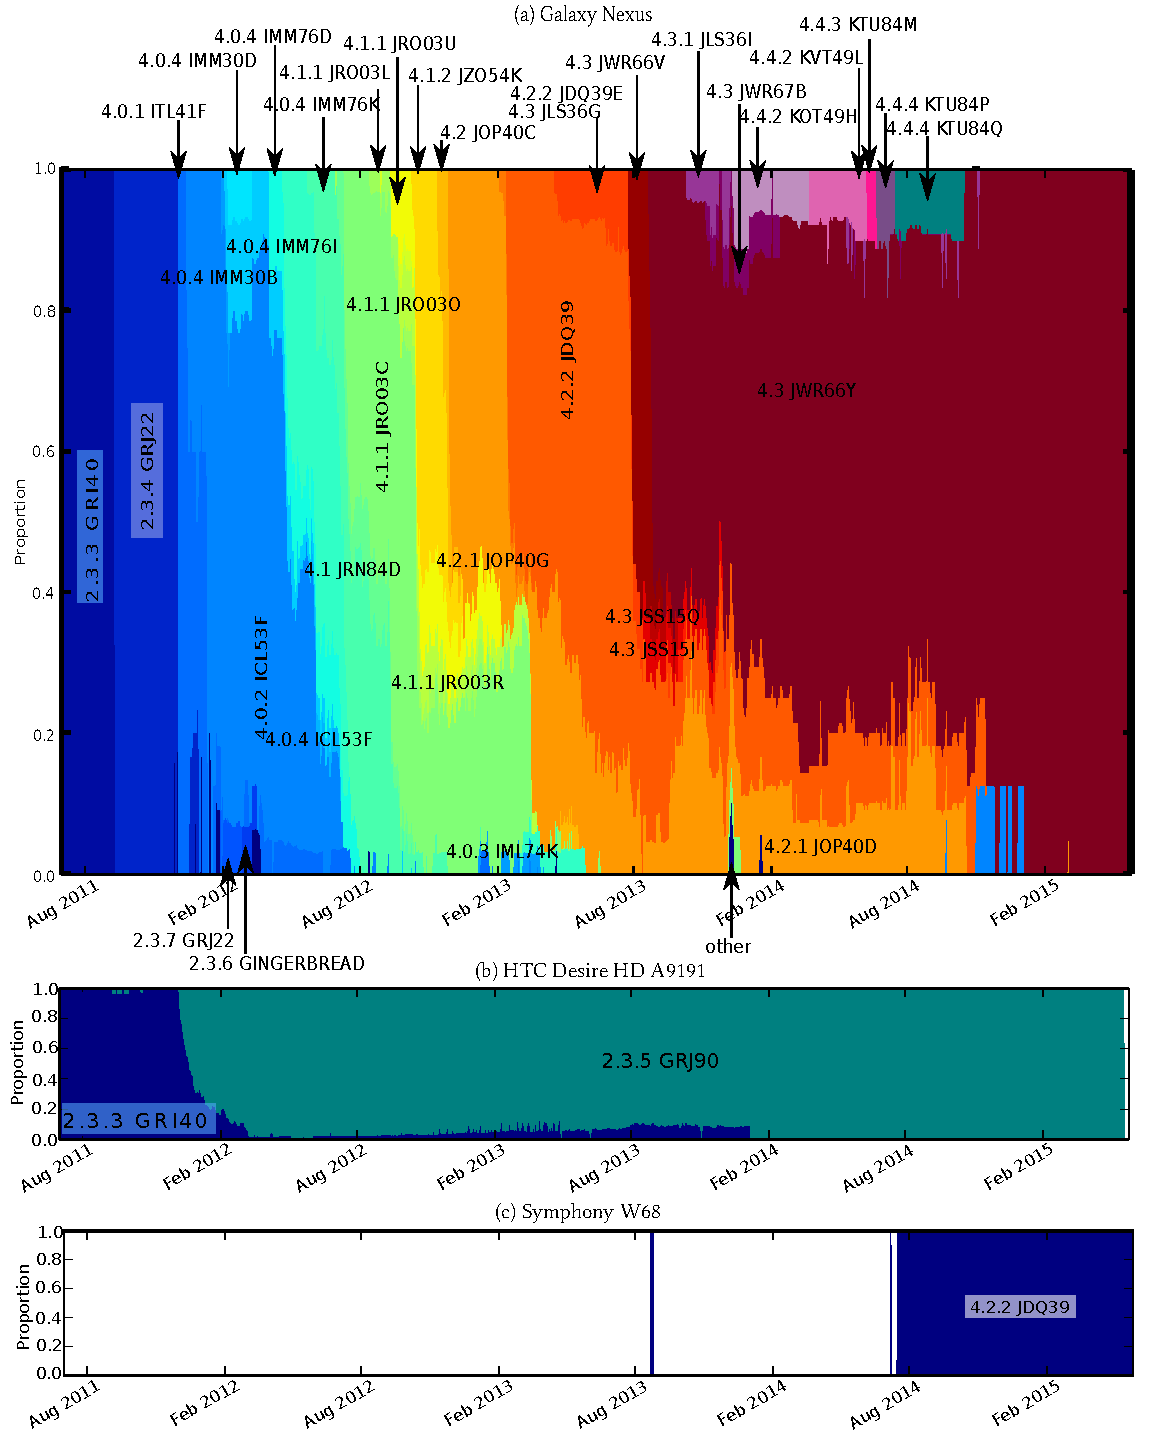
\includegraphics[width=0.9\textwidth]{figures/full_version_comp.pdf}
 \caption{Full version distributions for the highest and lowest scoring models}
 \label{fig:full_version_comp}
\end{figure*}

\daTabSecScoresoperator
We also analysed different network operators, for the \daNumSigOperators\ network operators with a significant presence in our data.
Table~\ref{tab:sec_operator} shows the results \emph{\daSecScoreBestoperator} (\daSecScoreBestoperatorScore\ out of 10) scoring highest and \emph{\daSecScoreWorstoperator} (\daSecScoreWorstoperatorScore\ out of 10) scoring lowest.
However the score of a network operator is affected by the device manufacturers of the devices which are in use on its network.
This is in turn affected by both what devices a network operator offers to users and upon which devices users choose.
Hence having a worse score does not necessarily mean that a network operator is worse, it could be that its users all pick phones from a worse device manufacturer, for example because they were cheaper.
A network operator could use data from this paper to exclude insecure devices from those offered to consumers.
An added value analysis of network operators which takes into account the device mix used by users of that network operator would make it possible to determine whether a network operator is making the situation better or worse by the way it ships updates to users.
However our sample size is too small to do that as while we have significant numbers of devices for each of the device models (Table~\ref{tab:sec_model}) and for each of the network operators (Table~\ref{tab:sec_operator}) we would need a significant number of each model in each network operator.
%We do not attempt to disambiguate users behaviour in whether they install updates from network operators using rolling upgrades.


\subsection{Scores over time}
\begin{figure}
\centering
\begin{subfigure}{\columnwidth}
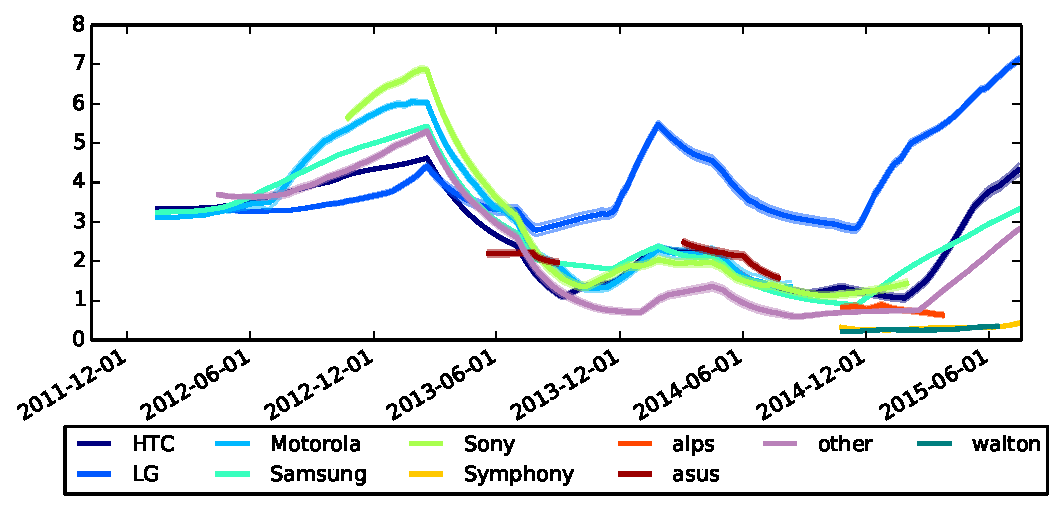
\includegraphics[width=\columnwidth]{figures/security_score_manufacturer}
\caption{Device manufacturers}
\label{fig:security_score_manufacturer}
\end{subfigure}
%
\begin{subfigure}{\columnwidth}
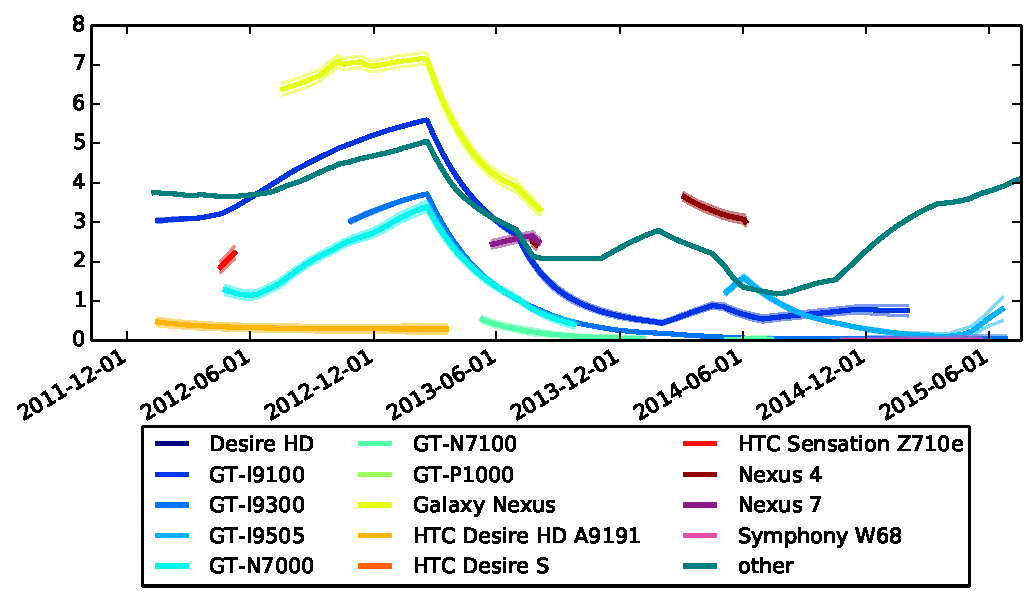
\includegraphics[width=\columnwidth]{figures/security_score_model}
\caption{Device models}
\label{fig:security_score_model}
\end{subfigure}
%
\begin{subfigure}{\columnwidth}
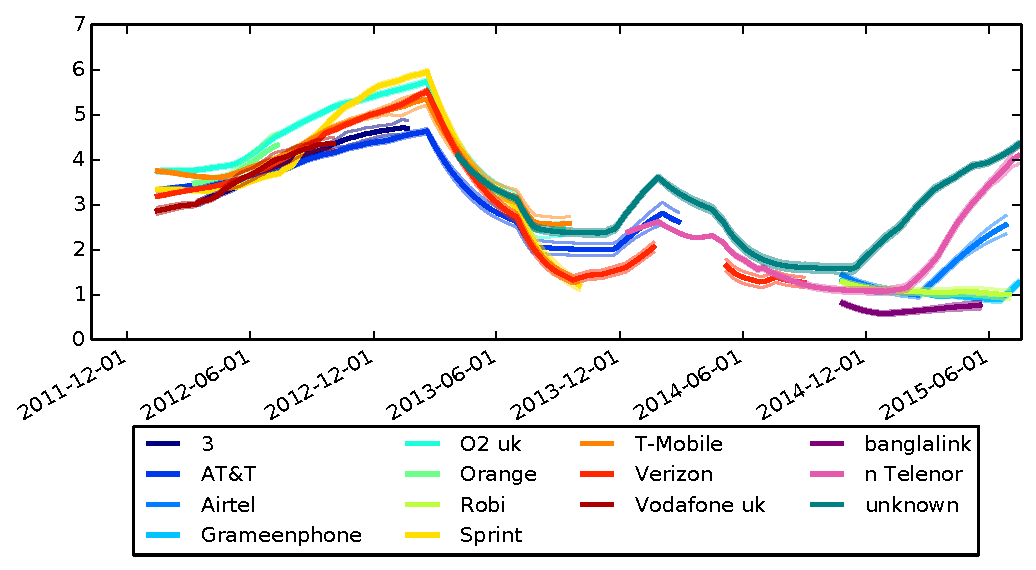
\includegraphics[width=\columnwidth]{figures/security_score_operator}
\caption{Network operators}
\label{fig:security_score_operator}
\end{subfigure}
%
\begin{subfigure}{\columnwidth}
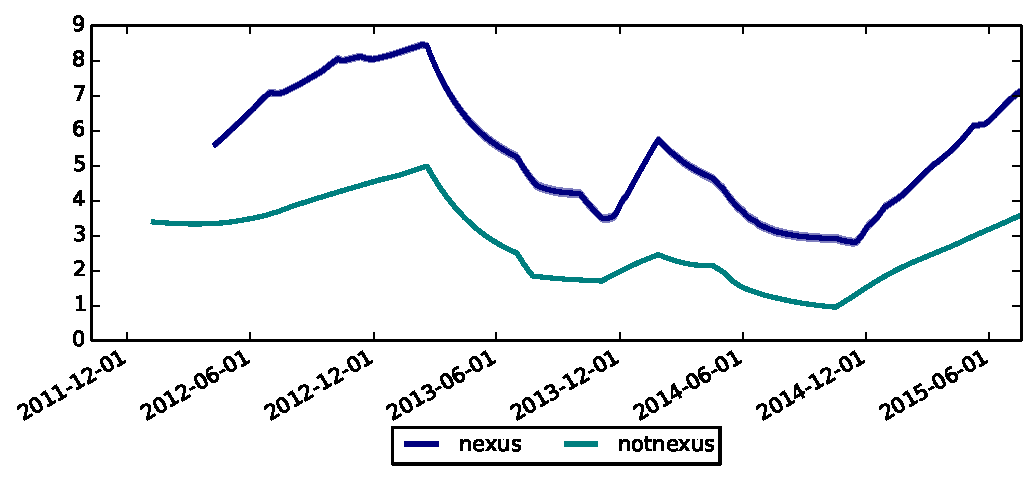
\includegraphics[width=\columnwidth]{figures/security_score_summary}
\caption{Nexus and non-Nexus devices}
\label{fig:security_score_summary}
\end{subfigure}
\caption{Security scores for device manufacturers, device models, network operators and Nexus devices. 95\% confidence intervals indicated.\todolater{bridge gaps?}}
\label{fig:security_scores}
\end{figure}
\todo{This is method rather than result}
The scoring metric as originally computed is averaged over the whole history of the device manufacturer, device model or network operator, it gives equal weight to periods years ago as to in the last few months.
If instead we take an exponential moving average of the daily score for days with more than \daSigNumDevicesDay\ devices when there have been at least consecutive \daSigNumDays\ days of data with that many devices then we can plot how this score has changed over time.
Equation~\ref{eq:rolling_update} shows how the value for a particular day ($v_i$) is computed from the previous day's value and the input for the current day ($n$) with an $\alpha$ of $1/\daSigNumDays$.
\begin{equation}
v_i = v_{i-1} (1 - \alpha) + n \alpha
\label{eq:rolling_update}
\end{equation}
Figure~\ref{fig:security_scores} shows this for manufacturers, device models, network operators and for Nexus and non-Nexus devices.
These show how the scores for different entities are different and change over time, while there is correlated behaviour for different entities (due to things like new vulnerabilities affecting all Android being discovered) these lines still have crossings due to the different behaviour of the different entities.
It also shows that we do not have sufficient data for all the entities all of the time, resulting in gaps in the data.
The clearest results are for Figure~\ref{fig:security_score_summary} with a large gap between the scores for Nexus and non-Nexus devices across the whole data set.


\subsection{Sensitivity of scoring metric}
\daTabDLDistances
\daTabChangeInScores
To evaluate whether the ranking of different manufacturers is sensitive to the form of the scoring metric we computed the normalised Damerau-Levenshtein distance~\cite{Bard2007} between the lists ordered using different forms of the scoring metric, this is shown in Table~\ref{tab:dl_distances}.
The `equal' metric weights $f$, $u$ and $m$ equally rather than favouring $f$ and makes little difference.
Changing the scoring metric also impacts the scores given for each entity Table~\ref{tab:change_in_scores} shows the mean impact on the scores.
This shows that $m$ tends to drag down scores.
\todo{Give some of the actual orderings as well for the most important ones}
\todo{Sensitivity of time based vs. global scores}

\subsection{Gaming the score}
If the comparative data given here is used to influence purchasing decisions then entities in the Android ecosystem might try to game the score rather than genuinely improve security.
$f$ is hard to game without doing a good job at security but it doesn't get any worse if there is already one known vulnerability and another is found.
A high value of $u$ could be achieved by only ever shipping one version but that would give low values for $f$ and $m$ (and not be attractive to new customers).
A high value of $m$ could be achieved by focusing on only one device at a time and ensuring that it gets updates but ignoring all others, but that would lower $f$ and $u$.%
One way to influence our scores would be to add additional devices to Device Analyzer which have good security, these would have to be real end user devices as we could detect fake ones, this would increase the size of our data set and would require providing genuinely good security to some users.
Therefore our score is secure against passive gaming attacks which changed the measured distribution but would require active defence against active gaming attacks which target the measurement devices.